% Converted from PBS_Deployment_Guide.md; original content retained.
% Compile in this directory: pdflatex PBS_Deployment_Guide.tex (twice).
% Keep PBS_Deployment_Guide_assets/ beside this source.
% Options for packages loaded elsewhere
\PassOptionsToPackage{unicode}{hyperref}
\PassOptionsToPackage{hyphens}{url}
\PassOptionsToPackage{dvipsnames,svgnames,x11names}{xcolor}
%
\documentclass[
  11pt,
  a4paper,
]{article}
\usepackage{amsmath,amssymb}
\usepackage{setspace}
\usepackage{iftex}
\ifPDFTeX
  \usepackage[T1]{fontenc}
  \usepackage[utf8]{inputenc}
  \usepackage{textcomp} % provide euro and other symbols
\else % if luatex or xetex
  \usepackage{unicode-math} % this also loads fontspec
  \defaultfontfeatures{Scale=MatchLowercase}
  \defaultfontfeatures[\rmfamily]{Ligatures=TeX,Scale=1}
\fi
\usepackage{lmodern}
\ifPDFTeX\else
  % xetex/luatex font selection
\fi
% Use upquote if available, for straight quotes in verbatim environments
\IfFileExists{upquote.sty}{\usepackage{upquote}}{}
\IfFileExists{microtype.sty}{% use microtype if available
  \usepackage[]{microtype}
  \UseMicrotypeSet[protrusion]{basicmath} % disable protrusion for tt fonts
}{}
\makeatletter
\@ifundefined{KOMAClassName}{% if non-KOMA class
  \IfFileExists{parskip.sty}{%
    \usepackage{parskip}
  }{% else
    \setlength{\parindent}{0pt}
    \setlength{\parskip}{6pt plus 2pt minus 1pt}}
}{% if KOMA class
  \KOMAoptions{parskip=half}}
\makeatother
\usepackage{xcolor}
\usepackage[margin=20mm]{geometry}
\usepackage{color}
\usepackage{fancyvrb}
\newcommand{\VerbBar}{|}
\newcommand{\VERB}{\Verb[commandchars=\\\{\}]}
\DefineVerbatimEnvironment{Highlighting}{Verbatim}{commandchars=\\\{\}}
% Add ',fontsize=\small' for more characters per line
\newenvironment{Shaded}{}{}
\newcommand{\AlertTok}[1]{\textcolor[rgb]{1.00,0.00,0.00}{\textbf{#1}}}
\newcommand{\AnnotationTok}[1]{\textcolor[rgb]{0.38,0.63,0.69}{\textbf{\textit{#1}}}}
\newcommand{\AttributeTok}[1]{\textcolor[rgb]{0.49,0.56,0.16}{#1}}
\newcommand{\BaseNTok}[1]{\textcolor[rgb]{0.25,0.63,0.44}{#1}}
\newcommand{\BuiltInTok}[1]{\textcolor[rgb]{0.00,0.50,0.00}{#1}}
\newcommand{\CharTok}[1]{\textcolor[rgb]{0.25,0.44,0.63}{#1}}
\newcommand{\CommentTok}[1]{\textcolor[rgb]{0.38,0.63,0.69}{\textit{#1}}}
\newcommand{\CommentVarTok}[1]{\textcolor[rgb]{0.38,0.63,0.69}{\textbf{\textit{#1}}}}
\newcommand{\ConstantTok}[1]{\textcolor[rgb]{0.53,0.00,0.00}{#1}}
\newcommand{\ControlFlowTok}[1]{\textcolor[rgb]{0.00,0.44,0.13}{\textbf{#1}}}
\newcommand{\DataTypeTok}[1]{\textcolor[rgb]{0.56,0.13,0.00}{#1}}
\newcommand{\DecValTok}[1]{\textcolor[rgb]{0.25,0.63,0.44}{#1}}
\newcommand{\DocumentationTok}[1]{\textcolor[rgb]{0.73,0.13,0.13}{\textit{#1}}}
\newcommand{\ErrorTok}[1]{\textcolor[rgb]{1.00,0.00,0.00}{\textbf{#1}}}
\newcommand{\ExtensionTok}[1]{#1}
\newcommand{\FloatTok}[1]{\textcolor[rgb]{0.25,0.63,0.44}{#1}}
\newcommand{\FunctionTok}[1]{\textcolor[rgb]{0.02,0.16,0.49}{#1}}
\newcommand{\ImportTok}[1]{\textcolor[rgb]{0.00,0.50,0.00}{\textbf{#1}}}
\newcommand{\InformationTok}[1]{\textcolor[rgb]{0.38,0.63,0.69}{\textbf{\textit{#1}}}}
\newcommand{\KeywordTok}[1]{\textcolor[rgb]{0.00,0.44,0.13}{\textbf{#1}}}
\newcommand{\NormalTok}[1]{#1}
\newcommand{\OperatorTok}[1]{\textcolor[rgb]{0.40,0.40,0.40}{#1}}
\newcommand{\OtherTok}[1]{\textcolor[rgb]{0.00,0.44,0.13}{#1}}
\newcommand{\PreprocessorTok}[1]{\textcolor[rgb]{0.74,0.48,0.00}{#1}}
\newcommand{\RegionMarkerTok}[1]{#1}
\newcommand{\SpecialCharTok}[1]{\textcolor[rgb]{0.25,0.44,0.63}{#1}}
\newcommand{\SpecialStringTok}[1]{\textcolor[rgb]{0.73,0.40,0.53}{#1}}
\newcommand{\StringTok}[1]{\textcolor[rgb]{0.25,0.44,0.63}{#1}}
\newcommand{\VariableTok}[1]{\textcolor[rgb]{0.10,0.09,0.49}{#1}}
\newcommand{\VerbatimStringTok}[1]{\textcolor[rgb]{0.25,0.44,0.63}{#1}}
\newcommand{\WarningTok}[1]{\textcolor[rgb]{0.38,0.63,0.69}{\textbf{\textit{#1}}}}
\usepackage{longtable,booktabs,array}
\usepackage{calc} % for calculating minipage widths
% Correct order of tables after \paragraph or \subparagraph
\usepackage{etoolbox}
\makeatletter
\patchcmd\longtable{\par}{\if@noskipsec\mbox{}\fi\par}{}{}
\makeatother
% Allow footnotes in longtable head/foot
\IfFileExists{footnotehyper.sty}{\usepackage{footnotehyper}}{\usepackage{footnote}}
\makesavenoteenv{longtable}
\setlength{\emergencystretch}{3em} % prevent overfull lines
\providecommand{\tightlist}{%
  \setlength{\itemsep}{0pt}\setlength{\parskip}{0pt}}
\setcounter{secnumdepth}{-\maxdimen} % remove section numbering
% Markdown-inspired typography; compile with pdfLaTeX from this directory.
\usepackage{graphicx}
\usepackage{tgheros}
\usepackage[scale=1.0]{inconsolata}
\renewcommand{\familydefault}{\sfdefault}
\usepackage{seqsplit}
\DeclareRobustCommand{\InlineCode}[1]{{\ttfamily\upshape\seqsplit{#1}}}
\usepackage{titlesec}
\usepackage{needspace}
\definecolor{MarkdownText}{HTML}{24292F}
\definecolor{MarkdownRule}{HTML}{D0D7DE}
\definecolor{shadecolor}{HTML}{F6F8FA}
\color{MarkdownText}
\titleformat{\section}{\LARGE\bfseries\raggedright}{}{0pt}{}[\color{MarkdownRule}\titlerule]
\titleformat{\subsection}{\Large\bfseries\raggedright}{}{0pt}{}[\color{MarkdownRule}\titlerule]
\titleformat{\subsubsection}{\large\bfseries\raggedright}{}{0pt}{}
\titlespacing*{\section}{0pt}{1.3em}{0.7em}
\titlespacing*{\subsection}{0pt}{1.2em}{0.6em}
\titlespacing*{\subsubsection}{0pt}{1em}{0.4em}
\setlength{\parindent}{0pt}
\setlength{\parskip}{0.55em plus 0.1em minus 0.1em}
\renewcommand{\arraystretch}{1.18}
\setlength{\tabcolsep}{5pt}
\setlength{\emergencystretch}{3em}
\raggedright
\raggedbottom
\widowpenalty=10000
\clubpenalty=10000
\usepackage{framed}
\renewenvironment{Shaded}{\begin{snugshade}}{\end{snugshade}}
\renewcommand{\CommentTok}[1]{\textcolor[rgb]{0.38,0.63,0.69}{#1}}
\usepackage{fvextra}
\fvset{breaklines=true,breakanywhere=true,fontsize=\small}
\DefineVerbatimEnvironment{verbatim}{Verbatim}{breaklines=true,breakanywhere=true,fontsize=\small}
\BeforeBeginEnvironment{verbatim}{\begin{snugshade}}
\AfterEndEnvironment{verbatim}{\end{snugshade}}
\AtBeginEnvironment{longtable}{\small}
\AtBeginDocument{\pdfstringdefDisableCommands{\def\InlineCode#1{#1}}}

\usepackage{pmboxdraw}
\ifLuaTeX
  \usepackage{selnolig}  % disable illegal ligatures
\fi
\IfFileExists{bookmark.sty}{\usepackage{bookmark}}{\usepackage{hyperref}}
\IfFileExists{xurl.sty}{\usepackage{xurl}}{} % add URL line breaks if available
\urlstyle{same}
\hypersetup{
  colorlinks=true,
  linkcolor={blue},
  filecolor={Maroon},
  citecolor={Blue},
  urlcolor={blue},
  pdfcreator={LaTeX via pandoc}}

\author{}
\date{}

\begin{document}

\setstretch{1.06}
\hypertarget{running-um-bridge-on-a-pbs-cluster-with-the-load-balancer-on-a-login-node}{%
\section{Running UM-Bridge on a PBS cluster with the load balancer on a
login
node}\label{running-um-bridge-on-a-pbs-cluster-with-the-load-balancer-on-a-login-node}}

This guide describes the implementation in this checkout of
\href{LoadBalancer.cpp}{\InlineCode{LoadBalancer.cpp}} and
\href{LoadBalancer.hpp}{\InlineCode{LoadBalancer.hpp}}, and the
accompanying PBS model-server script,
\href{job.sh}{\InlineCode{job.sh}}. It is intended to be followed from
preparation through a first evaluation, then used as an operations and
troubleshooting reference. The implementation and documentation were
reviewed on 31 October 2026.

The deployment has three roles: a client submits numerical requests; a
\InlineCode{LoadBalancer} process on one login node accepts those
requests; and PBS starts the actual model servers on compute nodes. This
arrangement follows the general
\href{https://um-bridge-benchmarks.readthedocs.io/en/docs/umbridge/hpc.html}{UM-Bridge
HPC architecture}. The direct \InlineCode{--scheduler=pbs}
implementation described here is a local extension; the upstream
instructions primarily describe direct SLURM submission and HyperQueue,
which can itself request PBS allocations.

The examples use \textbf{\InlineCode{testmodel} as both the executable
filename and the model name advertised through the UM-Bridge API}. They
are separate names. The build instructions deliberately make a demo that
uses both. Replace them with your own executable and advertised model
name when deploying a real application.

The guide assumes PBS Professional/OpenPBS-style resource directives, a
shared filesystem, and permission to run a lightweight HTTP service on
the login node. Queue names, account names, resource requests, module
setup, network names, and login-session management must be adapted to
the cluster. No real PBS submission is required merely to build the
software or read \InlineCode{--help}.

To rehearse everything on a multicore PC without PBS, see
\protect\hyperlink{rehearsal-on-your-own-pc-with-the-fake-pbs-commands}{Section
13}.

\hypertarget{deployment-overview-and-terminology}{%
\subsection{1. Deployment overview and
terminology}\label{deployment-overview-and-terminology}}

\begin{center}
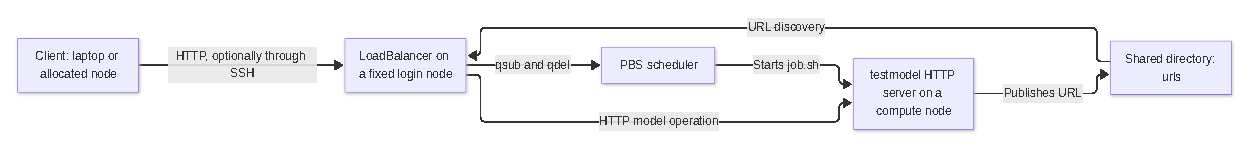
\includegraphics[width=\linewidth,height=0.78\textheight,keepaspectratio]{PBS_Deployment_Guide_assets/diagram-1.pdf}
\end{center}

There are two HTTP connections to arrange. The client must reach the
login-node listener, normally on port \InlineCode{4242}. Independently,
the login node must reach the compute-node model server on the port
selected by \InlineCode{job.sh}. An SSH tunnel for the first connection
does not establish the second connection. The shared filesystem carries
a small URL announcement; numerical inputs and outputs travel through
HTTP.

\Needspace{23\baselineskip}
\begin{longtable}[]{@{}
  >{\raggedright\arraybackslash}p{(\columnwidth - 4\tabcolsep) * \real{0.2300}}
  >{\raggedright\arraybackslash}p{(\columnwidth - 4\tabcolsep) * \real{0.4000}}
  >{\raggedright\arraybackslash}p{(\columnwidth - 4\tabcolsep) * \real{0.3700}}@{}}
\toprule\noalign{}
\begin{minipage}[b]{\linewidth}\raggedright
Name in this guide
\end{minipage} & \begin{minipage}[b]{\linewidth}\raggedright
Meaning
\end{minipage} & \begin{minipage}[b]{\linewidth}\raggedright
Where it is used
\end{minipage} \\
\midrule\noalign{}
\endhead
\bottomrule\noalign{}
\endlastfoot
\InlineCode{LoadBalancer} & The login-node executable, with this exact
capitalization & Built by the local HPC Makefile \\
\InlineCode{testmodel} executable & A program that serves the UM-Bridge
HTTP protocol & \InlineCode{model\_command=(./testmodel)} in
\InlineCode{job.sh} \\
\InlineCode{testmodel} API name & The name of a numerical model inside
that server & Client model selection and JSON \InlineCode{name}
fields \\
\InlineCode{testmodel} PBS job name & A readable scheduler label &
\InlineCode{\#PBS\space{}-N\space{}testmodel}; it does not set either
name above \\
Public port & Stable port on the login node &
\InlineCode{LoadBalancer\space{}--port=4242} \\
Backend port & A separate port chosen inside each allocation & Exported
as \InlineCode{PORT} before starting \InlineCode{testmodel} \\
Full PBS job ID & Scheduler identifier, for example
\InlineCode{12345.pbs01} & PBS diagnostics and manual cancellation \\
Numeric job ID & \InlineCode{12345} in the preceding example & This
implementation's URL filename and automatic \InlineCode{qdel} command \\
\end{longtable}

A UM-Bridge server may advertise several models. A model exposes
input/output dimensions, evaluation, and optional derivative operations.
The general programming interface is described in the
\href{https://um-bridge-benchmarks.readthedocs.io/en/docs/umbridge/models.html}{official
model documentation}. The deployment-specific behavior below comes from
the local C++ sources.

\hypertarget{existing-sample-names-require-attention}{%
\subsubsection{Existing sample names require
attention}\label{existing-sample-names-require-attention}}

This directory contains a ready-made demo model,
\href{testmodel.cpp}{\InlineCode{testmodel.cpp}}, which registers the
API name \InlineCode{"testmodel"}, and a prototype client,
\href{http-client.cpp}{\InlineCode{http-client.cpp}}, which requests
\InlineCode{"testmodel"}. The older sandbox pair one level up
(\href{../minimal-server.cpp}{\InlineCode{../minimal-server.cpp}} and
\href{../http-client.cpp}{\InlineCode{../http-client.cpp}}) registers
and selects \InlineCode{"forward"} instead; do not mix the two pairs.
Renaming an executable file does not change the API name compiled into
it. The Python and \InlineCode{curl} examples in this guide use
\InlineCode{testmodel}.

All four programs of this directory (\InlineCode{LoadBalancer},
\InlineCode{is\_port\_free}, \InlineCode{testmodel},
\InlineCode{http-client}) are built by the supplied
\InlineCode{Makefile}; see Section 4.

The demo model accepts one vector with two entries and computes
\InlineCode{2*x[0]\space{}+\space{}3*x[1]}. Thus
\InlineCode{[[100.0,\space{}18.0]]} produces \InlineCode{[[254.0]]}. The
official downloadable/container test model has a different example
contract; do not substitute its input dimensions for those of the
sandbox demo.

\hypertarget{what-the-local-load-balancer-actually-does}{%
\subsection{2. What the local load balancer actually
does}\label{what-the-local-load-balancer-actually-does}}

\hypertarget{initial-discovery-happens-before-the-login-node-listener-starts}{%
\subsubsection{2.1 Initial discovery happens before the login-node
listener
starts}\label{initial-discovery-happens-before-the-login-node-listener-starts}}

For \InlineCode{--scheduler=pbs}, \InlineCode{main()} performs the
following steps:

\begin{enumerate}
\def\labelenumi{\arabic{enumi}.}
\tightlist
\item
  Validate command-line options.
\item
  Remove existing regular files named \InlineCode{urls/url-<digits>.txt}
  in its working directory.
\item
  Construct a \InlineCode{PBSSubmitter}, a filesystem communicator
  factory, and a script locator using the relative directory
  \InlineCode{pbs\_scripts}.
\item
  Submit \textbf{one real PBS job} using the default
  \InlineCode{pbs\_scripts/job.sh}.
\item
  Poll for that job's URL announcement, query the backend
  \InlineCode{/Info}, and collect the model names it advertises.
\item
  Request cancellation of the discovery job and remove its URL
  announcement.
\item
  Create a proxy for each discovered model and start the public HTTP
  listener.
\end{enumerate}

Consequently, the public port can remain unavailable while the discovery
job is queued. The messages about a URL file and the job's state in
\InlineCode{qstat} are more useful at that stage than repeatedly trying
the public endpoint. Model names are discovered once at startup; restart
the balancer after changing the set of advertised models.

\hypertarget{a-model-operation-acquires-a-fresh-pbs-job}{%
\subsubsection{2.2 A model operation acquires a fresh PBS
job}\label{a-model-operation-acquires-a-fresh-pbs-job}}

\begin{center}
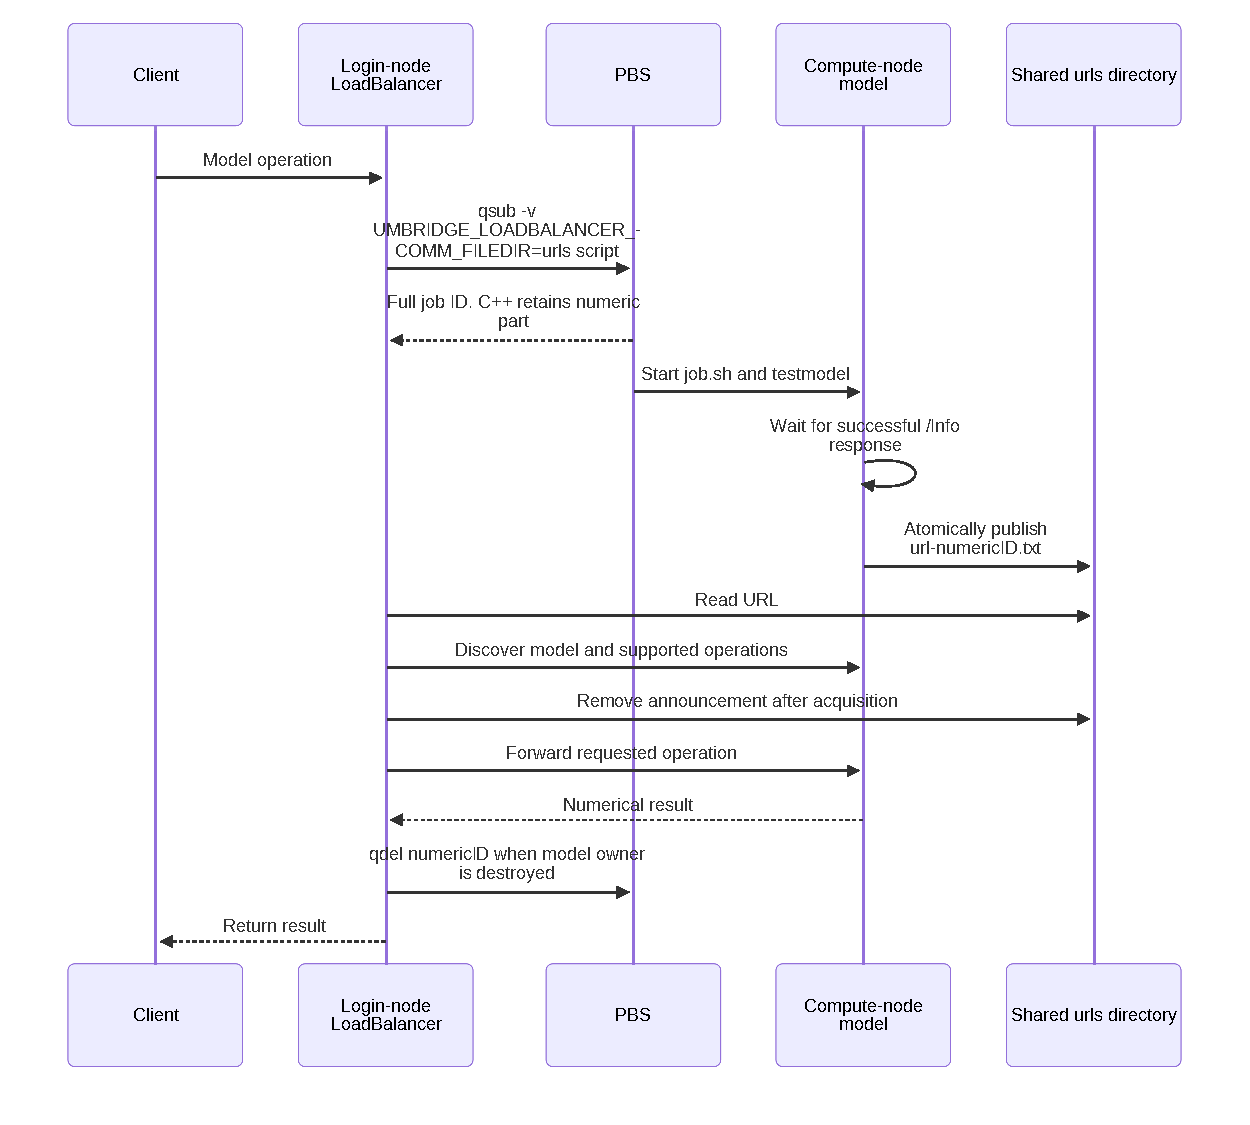
\includegraphics[width=\linewidth,height=0.78\textheight,keepaspectratio]{PBS_Deployment_Guide_assets/diagram-2.pdf}
\end{center}

\InlineCode{CommandJobManager::requestModelAccess()} creates a
communicator, submits a script, reads its URL, and constructs an
\InlineCode{umbridge::HTTPModel}. A \InlineCode{JobModel} keeps the
scheduler job alive while the requested operation runs. Destruction of
that owner invokes \InlineCode{qdel} through \InlineCode{PBSJob}. Normal
exception unwinding also releases already-owned jobs.

This applies to evaluation, derivatives, size queries, and support
queries. There is no retained backend pool, result cache, or metadata
cache in \InlineCode{LoadBalancer}. A backend HTTP client's discovery
calls happen within the job already being acquired; they do not
recursively submit more PBS jobs.

The public server allows concurrent requests. Each acquisition has its
own job and communicator, while PBS decides when resources become
available. The load balancer does not impose a maximum number of queued
or running jobs.

\hypertarget{metadata-has-a-scheduling-cost}{%
\subsubsection{2.3 Metadata has a scheduling
cost}\label{metadata-has-a-scheduling-cost}}

With the bundled
\href{../../../umbridge/lib/umbridge.h}{\InlineCode{umbridge.h}}, the
following costs follow from its HTTP handlers and the local proxy
methods:

\begin{longtable}[]{@{}
  >{\raggedright\arraybackslash}p{(\columnwidth - 2\tabcolsep) * \real{0.5500}}
  >{\raggedleft\arraybackslash}p{(\columnwidth - 2\tabcolsep) * \real{0.4500}}@{}}
\toprule\noalign{}
\begin{minipage}[b]{\linewidth}\raggedright
Request to the login-node balancer
\end{minipage} & \begin{minipage}[b]{\linewidth}\raggedleft
New PBS jobs after startup
\end{minipage} \\
\midrule\noalign{}
\endhead
\bottomrule\noalign{}
\endlastfoot
\InlineCode{GET\space{}/Info} & 0 \\
\InlineCode{POST\space{}/ModelInfo} & 4: one for each support query \\
\InlineCode{POST\space{}/InputSizes} & 1 \\
\InlineCode{POST\space{}/OutputSizes} & 1 \\
One evaluation & 1 \\
One supported Jacobian action & 1 \\
\end{longtable}

Use \InlineCode{/Info} for a lightweight service-liveness check.
Creating a high-level client object may request \InlineCode{/ModelInfo};
it is not necessarily a cheap local operation. For example, the
prototype C++ client's normal path without Jacobian support creates ten
jobs after startup: four support checks, four size queries across its
two configurations, and two evaluations. The startup discovery adds
another job. These counts describe this checkout, not a promise about
every UM-Bridge version or client implementation.

\hypertarget{prerequisites-and-compatibility-checks}{%
\subsection{3. Prerequisites and compatibility
checks}\label{prerequisites-and-compatibility-checks}}

\hypertarget{shared-storage-and-software}{%
\subsubsection{3.1 Shared storage and
software}\label{shared-storage-and-software}}

Choose a project directory visible under the same path from the login
and compute nodes. The model executable, its libraries/data, the helper
executable, the job script, and \InlineCode{urls} must be accessible
there. The script explicitly returns to the submission directory before
using relative paths.

The login node needs a C++20-capable compiler (the Makefile uses
\InlineCode{-std=c++20}) for building, GNU Make, real PBS client
commands, and the bundled UM-Bridge headers. The supplied Makefiles link
OpenSSL; install/load the cluster's OpenSSL development environment as
needed. Compute nodes need Bash, \InlineCode{curl}, \InlineCode{shuf},
\InlineCode{hostname}, \InlineCode{mktemp}, standard file utilities, and
the runtime libraries required by the compiled model and helper. Load
compiler, MPI, Python, or container modules in the job script if the
model depends on them. A module loaded in an interactive login shell
does not by itself document or reproduce the compute job's environment.

\hypertarget{make-sure-the-commands-are-real-pbs-commands}{%
\subsubsection{3.2 Make sure the commands are real PBS
commands}\label{make-sure-the-commands-are-real-pbs-commands}}

On the login node, inspect:

\Needspace{5\baselineskip}

\begin{Shaded}
\begin{Highlighting}[]
\BuiltInTok{type} \AttributeTok{{-}a}\NormalTok{ qsub qstat qdel}
\BuiltInTok{command} \AttributeTok{{-}v}\NormalTok{ qsub}
\BuiltInTok{command} \AttributeTok{{-}v}\NormalTok{ qdel}
\end{Highlighting}
\end{Shaded}

The subfolder \InlineCode{hpc/bin} contains fake \InlineCode{qsub},
\InlineCode{qstat} and \InlineCode{qdel} scripts for rehearsing on a PC
without PBS (Section 13). They are kept apart from the deployment
directory precisely so that they cannot shadow the real commands:
\textbf{on the cluster, never put \InlineCode{hpc/bin} in
\InlineCode{PATH}.} The C++ code invokes the bare command names through
a shell; shell aliases and interactive functions are not a reliable way
to choose the scheduler binary. Use the site's PBS environment/module
and verify the resolved executable paths.

The fake commands support \InlineCode{-v}, \InlineCode{PBS\_JOBID},
\InlineCode{PBS\_O\_WORKDIR} and \InlineCode{qdel} termination of the
whole job, so they permit an end-to-end test of the software logic, but
they say nothing about the cluster's queues, network or modules. Their
\InlineCode{MAX\_JOBS} setting has no effect on a real PBS scheduler.

\hypertarget{check-the-full-pbs-job-id-format-before-using-the-balancer}{%
\subsubsection{3.3 Check the full PBS job ID format before using the
balancer}\label{check-the-full-pbs-job-id-format-before-using-the-balancer}}

The current \InlineCode{PBSJob} parser accepts only:

\Needspace{5\baselineskip}

\begin{Shaded}
\begin{Highlighting}[]
\NormalTok{12345}
\NormalTok{12345.pbs01}
\NormalTok{12345.pbs{-}server\_1}
\end{Highlighting}
\end{Shaded}

The suffix may contain letters, digits, underscores, and hyphens. It
cannot contain a further dot. Forms such as
\InlineCode{12345.pbs.cluster.example}, array IDs, and
\InlineCode{12345.pbs01@other-server} are not accepted by this C++
implementation. The converted job script deliberately enforces the same
restriction.

Verify the format using a small manual job as described in section 6. If
the cluster emits an unsupported format, resolve the compatibility issue
before starting the balancer. A C++ parser/identifier-handling change
would be required for general support; editing only the filename in
\InlineCode{job.sh} is insufficient. Successful scheduler submission
followed by a parser error can leave a submitted job without a C++
owner. Inspect \InlineCode{qstat} and cancel such a job manually using
its full PBS ID.

Automatic cancellation uses only the numeric portion, for example
\InlineCode{qdel\space{}12345}. The PBS client environment must
therefore select the correct default server. The scheduler itself
supports broader identifiers than this local adapter; see the
\href{https://github.com/openpbs/openpbs/blob/master/doc/man1/qdel.1B}{OpenPBS
deletion command}.

\hypertarget{verify-the-network-paths}{%
\subsubsection{3.4 Verify the network
paths}\label{verify-the-network-paths}}

Confirm that the login node can resolve the compute-node hostname
advertised by the script and connect to the chosen backend TCP port. The
default script uses \InlineCode{hostname\space{}-f} and randomly selects
a port from \InlineCode{1024} through \InlineCode{65535}. If the cluster
permits only a restricted port range, change \InlineCode{port\_min} and
\InlineCode{port\_max} in the script to that range. If compute nodes
have several interfaces, set \InlineCode{advertise\_host} to the
name/address reachable from the login node.

The model must bind to a reachable interface, normally
\InlineCode{0.0.0.0}, rather than only its own loopback interface. Never
publish \InlineCode{localhost} or \InlineCode{127.0.0.1} as the
compute-node address: the login-node client would interpret that as the
login node itself. A readiness request made on the compute node is
useful but does not prove that login-to-compute routing or firewall
rules are correct.

The current public listener uses plain HTTP on
\InlineCode{0.0.0.0:<port>}. It has no command-line authentication, TLS,
or bind-address setting. Restrict access using the site's network
controls and supported service-hosting arrangement. A reachable caller
can trigger work submitted under the balancer's PBS identity. An SSH
tunnel protects and exposes the client-to-login connection; it does not
change the listener's bind address or add application authentication.

\hypertarget{prepare-the-directory-and-build-the-executables}{%
\subsection{4. Prepare the directory and build the
executables}\label{prepare-the-directory-and-build-the-executables}}

Use a shared checkout path in the following commands. Replace the
example value of \InlineCode{UMBRIDGE\_PROJECT} with the actual root
containing \InlineCode{sandbox} and \InlineCode{umbridge}. The path
should avoid whitespace and shell metacharacters; this adapter checks
raw script arguments before passing them to a shell.

\Needspace{6\baselineskip}

\begin{Shaded}
\begin{Highlighting}[]
\BuiltInTok{export} \VariableTok{UMBRIDGE\_PROJECT}\OperatorTok{=}\NormalTok{/shared/project/SparseGrid}
\BuiltInTok{cd} \StringTok{"}\VariableTok{$UMBRIDGE\_PROJECT}\StringTok{/sandbox/C++/hpc"}

\FunctionTok{make}
\end{Highlighting}
\end{Shaded}

The supplied \href{Makefile}{\InlineCode{Makefile}} builds all four
programs: \textbf{\InlineCode{LoadBalancer}} (not
\InlineCode{load-balancer}), the helper \InlineCode{is\_port\_free}, the
demo model \InlineCode{testmodel}, and the client
\InlineCode{http-client}. It compiles with C++20 and links OpenSSL
(\InlineCode{-lssl\space{}-lcrypto}), so the OpenSSL development package
must be installed. \InlineCode{make} rebuilds only what is out of date;
to build a single program, name it, for example
\InlineCode{make\space{}testmodel}. \InlineCode{make\space{}clean}
removes \InlineCode{LoadBalancer} and \InlineCode{is\_port\_free}. The
helper probes an IPv4 bind; it does not reserve the port after the
helper process exits.

The demonstration model is supplied in this directory as
\href{testmodel.cpp}{\InlineCode{testmodel.cpp}}: it registers the API
name \InlineCode{"testmodel"}, reads the listening port from the
\InlineCode{PORT} environment variable (default 4242) and an optional
artificial delay in milliseconds from \InlineCode{TEST\_DELAY}, and
computes \InlineCode{2*x[0]\space{}+\space{}3*x[1]}. It is compiled by
the \InlineCode{make} command above. If you adapt it, keep the name
passed to \InlineCode{umbridge::Model(...)} identical to the name your
client requests, and run \InlineCode{make\space{}testmodel} again after
every change. Then prepare the remaining directories and check that
everything is in place:

\Needspace{7\baselineskip}

\begin{Shaded}
\begin{Highlighting}[]
\FunctionTok{mkdir} \AttributeTok{{-}p}\NormalTok{ urls}
\BuiltInTok{test} \AttributeTok{{-}r}\NormalTok{ pbs\_scripts/job.sh}
\BuiltInTok{test} \AttributeTok{{-}x}\NormalTok{ ./testmodel}
\BuiltInTok{test} \AttributeTok{{-}x}\NormalTok{ ./is\_port\_free}
\ExtensionTok{./LoadBalancer} \AttributeTok{{-}{-}help}
\end{Highlighting}
\end{Shaded}

The resulting layout is:

\Needspace{19\baselineskip}

\begin{Shaded}
\begin{Highlighting}[]
\NormalTok{sandbox/C++/hpc/                 \textless{}{-} submission directory and balancer working directory}
\NormalTok{├── LoadBalancer                 \textless{}{-} login{-}node executable}
\NormalTok{├── LoadBalancer.cpp}
\NormalTok{├── LoadBalancer.hpp}
\NormalTok{├── bin/                         \textless{}{-} fake PBS commands, PC rehearsal only (Section 13)}
\NormalTok{│   ├── qsub}
\NormalTok{│   ├── qstat}
\NormalTok{│   ├── qdel}
\NormalTok{│   └── fakepbs{-}common.sh        \textless{}{-} helper sourced by the three commands}
\NormalTok{├── pbs\_scripts/}
\NormalTok{│   └── job.sh                   \textless{}{-} default script used by LoadBalancer}
\NormalTok{├── is\_port\_free                 \textless{}{-} compute{-}node helper}
\NormalTok{├── testmodel                    \textless{}{-} compute{-}node model executable}
\NormalTok{├── testmodel.cpp                \textless{}{-} demo model source (supplied)}
\NormalTok{├── http{-}client.cpp              \textless{}{-} prototype C++ client (supplied), see Section 8.4}
\NormalTok{├── http{-}client                  \textless{}{-} client executable, built in Section 8.4}
\NormalTok{└── urls/                        \textless{}{-} transient URL announcements}
\end{Highlighting}
\end{Shaded}

Do not launch two balancers in the same working directory. Startup
removes URL files matching the naming convention, and one instance can
delete another instance's announcements. A different public port alone
does not isolate the shared state. Give each independent deployment its
own working directory, \InlineCode{urls}, and script setup.

\hypertarget{configure-and-understand-the-pbs-model-job}{%
\subsection{5. Configure and understand the PBS model
job}\label{configure-and-understand-the-pbs-model-job}}

\hypertarget{resource-requests-and-customization-points}{%
\subsubsection{5.1 Resource requests and customization
points}\label{resource-requests-and-customization-points}}

The converted \href{pbs_scripts/job.sh}{\InlineCode{job.sh}} begins
with:

\Needspace{9\baselineskip}

\begin{Shaded}
\begin{Highlighting}[]
\CommentTok{\#!/bin/bash}
\CommentTok{\#PBS {-}S /bin/bash}
\CommentTok{\#PBS {-}N testmodel}
\CommentTok{\#PBS {-}l select=1:ncpus=1:mpiprocs=1:mem=1gb}
\CommentTok{\#PBS {-}l walltime=00:05:00}
\CommentTok{\#\#PBS {-}q CHANGE\_ME\_QUEUE}
\CommentTok{\#\#PBS {-}A CHANGE\_ME\_PROJECT}
\end{Highlighting}
\end{Shaded}

Change \InlineCode{\#\#PBS} to \InlineCode{\#PBS} only after replacing
the queue/account placeholder with a valid site value. The one-CPU,
one-GiB, five-minute allocation is a starting point for the tiny demo.
Allocate enough time for environment setup, server startup, the
requested operation, and normal teardown. Resource syntax and site
limits must match the installed scheduler; the chunk-resource
definitions are documented in the
\href{https://github.com/openpbs/openpbs/blob/master/doc/man1/pbs_resources.7B}{OpenPBS
resource manual}.

\begin{longtable}[]{@{}
  >{\raggedright\arraybackslash}p{(\columnwidth - 4\tabcolsep) * \real{0.2900}}
  >{\raggedright\arraybackslash}p{(\columnwidth - 4\tabcolsep) * \real{0.2300}}
  >{\raggedright\arraybackslash}p{(\columnwidth - 4\tabcolsep) * \real{0.4800}}@{}}
\toprule\noalign{}
\begin{minipage}[b]{\linewidth}\raggedright
Setting in \InlineCode{job.sh}
\end{minipage} & \begin{minipage}[b]{\linewidth}\raggedright
Default
\end{minipage} & \begin{minipage}[b]{\linewidth}\raggedright
What to change for your model
\end{minipage} \\
\midrule\noalign{}
\endhead
\bottomrule\noalign{}
\endlastfoot
\InlineCode{model\_command} & \InlineCode{(./testmodel)} & Executable
and arguments; use array entries to preserve argument boundaries \\
PBS \InlineCode{select} & One chunk, one CPU, one MPI process, 1 GiB &
CPU, memory, GPU, and node requirements supported by your site \\
PBS \InlineCode{walltime} & \InlineCode{00:05:00} & Longest expected
startup plus one operation, with margin \\
Queue/account directives & Commented placeholders & Site-required queue
and project/account \\
Module initialization & Commented edit point & Compiler, libraries, MPI,
Python environment, or container setup \\
\InlineCode{startup\_timeout\_seconds} & \InlineCode{120} & Time allowed
for backend readiness after the job starts running \\
\InlineCode{port\_min}, \InlineCode{port\_max} & \InlineCode{1024},
\InlineCode{65535} & A login-reachable, site-permitted TCP port range \\
\InlineCode{port\_attempts} & \InlineCode{100} & Maximum candidate ports
to probe \\
\InlineCode{advertise\_host} & Output of \InlineCode{hostname\space{}-f}
& Compute-node name reachable from the login node \\
\end{longtable}

LoadBalancer sends the equivalent of:

\Needspace{3\baselineskip}

\begin{Shaded}
\begin{Highlighting}[]
\ExtensionTok{qsub} \AttributeTok{{-}v} \StringTok{\textquotesingle{}UMBRIDGE\_LOADBALANCER\_COMM\_FILEDIR=urls\textquotesingle{}}\NormalTok{ pbs\_scripts/job.sh}
\end{Highlighting}
\end{Shaded}

The selected-variable export is intentional. The implementation does not
add \InlineCode{-V} or automatically forward arbitrary settings from the
login shell. Put application settings in the script, or explicitly
arrange their export using the site's PBS mechanisms. PBS provides
\InlineCode{PBS\_JOBID} and \InlineCode{PBS\_O\_WORKDIR};
\InlineCode{-v} supplies the URL-directory variable. See the
\href{https://github.com/openpbs/openpbs/blob/master/doc/man1/qsub.1B}{OpenPBS
submission manual}.

For example, setting \InlineCode{export\space{}TEST\_DELAY=2000} only in
your login shell is not a reliable way to configure this batch job. Add
the desired assignment in the job's environment-setup section if you are
using the sandbox demo's delay facility. Do not assume \InlineCode{PORT}
from the login shell controls the backend: the script deliberately
assigns it after selecting a port.

\hypertarget{what-the-converted-script-does}{%
\subsubsection{5.2 What the converted script
does}\label{what-the-converted-script-does}}

The script validates its required environment and runs
\InlineCode{cd\space{}"\$PBS\_O\_WORKDIR"}. It checks the full ID
against the adapter's supported format, extracts the numeric component,
and prepares the communication directory. This keeps
\InlineCode{./testmodel}, \InlineCode{./is\_port\_free}, and relative
\InlineCode{urls} anchored at the same shared directory that the
login-node balancer uses.

Next it selects a port, exports \InlineCode{PORT}, launches the model
command in the background, and records the process ID. It requests the
model's \InlineCode{/Info} endpoint with \InlineCode{curl}, bypassing
web proxies and requiring a successful HTTP status. The check has
bounded individual connection/request times and checks whether the model
process is still alive. Full UM-Bridge body/protocol validation follows
when the load balancer connects.

Once the server responds, the script writes a complete URL to a
temporary file in the communication directory and renames it to the
final filename. For \InlineCode{PBS\_JOBID=12345.pbs01}, the final
contents look like:

\Needspace{4\baselineskip}

\begin{Shaded}
\begin{Highlighting}[]
\NormalTok{\# filename: urls/url{-}12345.txt}
\NormalTok{http://compute017.cluster.internal:53017}
\end{Highlighting}
\end{Shaded}

The actual file contains only the URL line, without the explanatory
comment. The rename avoids exposing a newly created but empty
announcement to the balancer, which treats an empty line as an error.
Publication and final rename take place in the same shared directory.

Finally, the batch script waits for the model process. If the model
exits, the script ends; it does not remain in
\InlineCode{sleep\space{}infinity}. On termination, its trap attempts to
stop and reap the directly launched model process and remove an
unfinished temporary announcement. PBS manages the complete allocation
and its process tree. The script leaves removal of the final URL
announcement to the balancer's communicator.

\hypertarget{timeouts-liveness-and-file-lifetime}{%
\subsubsection{5.3 Timeouts, liveness, and file
lifetime}\label{timeouts-liveness-and-file-lifetime}}

The script's 120-second startup timer begins \textbf{after PBS starts
executing the job}, not while it waits in the queue. A bounded
\InlineCode{curl} attempt can make the observed cutoff slightly longer.
PBS walltime governs the running allocation.

The C++ balancer polls for the URL file every 500 ms with \textbf{no
overall timeout} and no \InlineCode{qstat} query. If the script fails
before publication, its new timeout or liveness check stops that job,
but the balancer can still wait forever for the missing file. Diagnose
and resolve such failures using the job state and logs; do not interpret
the script timeout as a timeout for the whole client request.

The URL file is a startup handshake. During normal acquisition, the
balancer removes it after constructing the HTTP model, even though the
job may still be running the numerical operation. Absence of a URL file
therefore does not prove that its job has finished. Use scheduler state
and logs to determine job status.

\hypertarget{pbs-standard-output-and-standard-error}{%
\subsubsection{5.4 PBS standard output and standard
error}\label{pbs-standard-output-and-standard-error}}

The template leaves PBS's per-job output and error destinations in
place. With the default job name, these are typically
\InlineCode{testmodel.o<sequence>} and
\InlineCode{testmodel.e<sequence>} in the submission directory, subject
to site settings. Their delivery or visibility during execution depends
on the site's spooling configuration.
\InlineCode{qstat\space{}-f\space{}<full-job-id>} shows the configured
output/error paths. The submission manual linked above describes
\InlineCode{-o} and \InlineCode{-e} overrides.

Do not write
\InlineCode{\#PBS\space{}-o\space{}output\_\$\{PBS\_JOBID\}} expecting
ordinary shell variable expansion: PBS processes directives before the
job shell executes. Avoid a single fixed log filename shared by all
jobs, because concurrent requests would overwrite or mix their logs. The
fake PBS of Section 13 follows the real default naming
(\InlineCode{<name>.o<id>}, \InlineCode{<name>.e<id>}) and honors
\InlineCode{-o}/\InlineCode{-e}, but it does not reproduce site spooling
behavior.

\hypertarget{test-one-backend-job-manually-before-starting-loadbalancer}{%
\subsection{6. Test one backend job manually before starting
LoadBalancer}\label{test-one-backend-job-manually-before-starting-loadbalancer}}

This test isolates scheduling, the batch environment, the model
executable, shared storage, and login-to-compute networking. Run it from
the deployment directory on the login node, using the real PBS commands:

\Needspace{8\baselineskip}

\begin{Shaded}
\begin{Highlighting}[]
\BuiltInTok{cd} \StringTok{"}\VariableTok{$UMBRIDGE\_PROJECT}\StringTok{/sandbox/C++/hpc"}
\FunctionTok{mkdir} \AttributeTok{{-}p}\NormalTok{ urls}

\VariableTok{pbs\_job\_id}\OperatorTok{=}\VariableTok{$(}\ExtensionTok{qsub} \AttributeTok{{-}v} \StringTok{\textquotesingle{}UMBRIDGE\_LOADBALANCER\_COMM\_FILEDIR=urls\textquotesingle{}}\NormalTok{ pbs\_scripts/job.sh}\VariableTok{)}
\BuiltInTok{printf} \StringTok{\textquotesingle{}Submitted PBS job: \%s\textbackslash{}n\textquotesingle{}} \StringTok{"}\VariableTok{$pbs\_job\_id}\StringTok{"}
\ExtensionTok{qstat} \AttributeTok{{-}f} \StringTok{"}\VariableTok{$pbs\_job\_id}\StringTok{"}
\end{Highlighting}
\end{Shaded}

Check the returned ID before continuing. Keep the complete string for
diagnostics and manual cancellation. For a supported ID such as
\InlineCode{12345.pbs01}, derive the handshake path as follows:

\Needspace{5\baselineskip}

\begin{Shaded}
\begin{Highlighting}[]
\VariableTok{numeric\_job\_id}\OperatorTok{=}\VariableTok{$\{pbs\_job\_id}\OperatorTok{\%\%}\NormalTok{.}\PreprocessorTok{*}\VariableTok{\}}
\VariableTok{url\_file}\OperatorTok{=}\StringTok{"urls/url{-}}\VariableTok{$\{numeric\_job\_id\}}\StringTok{.txt"}
\BuiltInTok{printf} \StringTok{\textquotesingle{}Expected URL file: \%s\textbackslash{}n\textquotesingle{}} \StringTok{"}\VariableTok{$url\_file}\StringTok{"}
\end{Highlighting}
\end{Shaded}

While the job is queued, no URL file is expected. Inspect
\InlineCode{qstat} and the PBS logs rather than assuming an application
failure. Once the job is running and the announcement exists:

\Needspace{13\baselineskip}

\begin{Shaded}
\begin{Highlighting}[]
\VariableTok{model\_url}\OperatorTok{=}\VariableTok{$(}\FunctionTok{head} \AttributeTok{{-}n}\NormalTok{ 1 }\StringTok{"}\VariableTok{$url\_file}\StringTok{"}\VariableTok{)}
\BuiltInTok{printf} \StringTok{\textquotesingle{}Backend address: \%s\textbackslash{}n\textquotesingle{}} \StringTok{"}\VariableTok{$model\_url}\StringTok{"}

\ExtensionTok{curl} \AttributeTok{{-}{-}fail} \AttributeTok{{-}{-}show{-}error} \AttributeTok{{-}{-}noproxy} \StringTok{\textquotesingle{}*\textquotesingle{}} \DataTypeTok{\textbackslash{}}
    \AttributeTok{{-}{-}connect{-}timeout}\NormalTok{ 5 }\AttributeTok{{-}{-}max{-}time}\NormalTok{ 15 }\StringTok{"}\VariableTok{$model\_url}\StringTok{/Info"}

\ExtensionTok{curl} \AttributeTok{{-}{-}fail} \AttributeTok{{-}{-}show{-}error} \AttributeTok{{-}{-}noproxy} \StringTok{\textquotesingle{}*\textquotesingle{}} \DataTypeTok{\textbackslash{}}
    \AttributeTok{{-}{-}connect{-}timeout}\NormalTok{ 5 }\AttributeTok{{-}{-}max{-}time}\NormalTok{ 30 }\DataTypeTok{\textbackslash{}}
    \AttributeTok{{-}H} \StringTok{\textquotesingle{}Content{-}Type: application/json\textquotesingle{}} \DataTypeTok{\textbackslash{}}
    \AttributeTok{{-}d} \StringTok{\textquotesingle{}\{"name":"testmodel","input":[[100.0,18.0]],"config":\{\}\}\textquotesingle{}} \DataTypeTok{\textbackslash{}}
    \StringTok{"}\VariableTok{$model\_url}\StringTok{/Evaluate"}
\end{Highlighting}
\end{Shaded}

For the renamed sandbox demo, \InlineCode{/Info} advertises
\InlineCode{testmodel}, and the evaluation contains
\InlineCode{"output":[[254.0]]} (numeric formatting may differ). If
\InlineCode{/Info} advertises \InlineCode{forward}, the executable was
built without changing its registered model name. Adapt the client name
or rebuild the intended demo.

These requests go directly to the one compute-node server. They do not
use the balancer or start additional jobs. After the test, cancel only
that job and remove its manual-test announcement:

\Needspace{4\baselineskip}

\begin{Shaded}
\begin{Highlighting}[]
\ExtensionTok{qdel} \StringTok{"}\VariableTok{$pbs\_job\_id}\StringTok{"}
\FunctionTok{rm} \AttributeTok{{-}f} \AttributeTok{{-}{-}} \StringTok{"}\VariableTok{$url\_file}\StringTok{"}
\end{Highlighting}
\end{Shaded}

If submission succeeded but the returned ID format is unsupported, use
its full ID to cancel it and fix the compatibility issue before
proceeding. If the backend test fails, resolve it here: the balancer
cannot repair an incorrect module environment, an unreachable compute
hostname, or a model that ignores the selected \InlineCode{PORT}.

\hypertarget{start-the-load-balancer-on-the-login-node}{%
\subsection{7. Start the load balancer on the login
node}\label{start-the-load-balancer-on-the-login-node}}

Record the specific login host, then start the process from the shared
deployment directory:

\Needspace{5\baselineskip}

\begin{Shaded}
\begin{Highlighting}[]
\BuiltInTok{cd} \StringTok{"}\VariableTok{$UMBRIDGE\_PROJECT}\StringTok{/sandbox/C++/hpc"}
\FunctionTok{hostname} \AttributeTok{{-}f}
\ExtensionTok{./LoadBalancer} \AttributeTok{{-}{-}scheduler}\OperatorTok{=}\NormalTok{pbs }\AttributeTok{{-}{-}port}\OperatorTok{=}\NormalTok{4242 }\AttributeTok{{-}{-}delay{-}ms}\OperatorTok{=}\NormalTok{0}
\end{Highlighting}
\end{Shaded}

Keep this foreground launch for the first test so startup messages are
visible. The expected sequence includes waiting for the discovery job's
URL file, then printing available model names and selected job scripts.
Initial availability depends on PBS queue time. In a second session on
the \textbf{same login node}, check:

\Needspace{4\baselineskip}

\begin{Shaded}
\begin{Highlighting}[]
\ExtensionTok{curl} \AttributeTok{{-}{-}fail} \AttributeTok{{-}{-}show{-}error} \AttributeTok{{-}{-}noproxy} \StringTok{\textquotesingle{}*\textquotesingle{}} \DataTypeTok{\textbackslash{}}
    \AttributeTok{{-}{-}connect{-}timeout}\NormalTok{ 5 }\AttributeTok{{-}{-}max{-}time}\NormalTok{ 15 http://127.0.0.1:4242/Info}
\end{Highlighting}
\end{Shaded}

After successful startup, this should report the \InlineCode{testmodel}
name without submitting another job. Verify endpoint reachability
explicitly: the bundled server does not give this \InlineCode{main()} a
reliable bind-success result to report. If another process already owns
port 4242, choose a different port and update the clients and tunnel
accordingly.

\begin{longtable}[]{@{}
  >{\raggedright\arraybackslash}p{(\columnwidth - 4\tabcolsep) * \real{0.3000}}
  >{\raggedright\arraybackslash}p{(\columnwidth - 4\tabcolsep) * \real{0.3000}}
  >{\raggedright\arraybackslash}p{(\columnwidth - 4\tabcolsep) * \real{0.4000}}@{}}
\toprule\noalign{}
\begin{minipage}[b]{\linewidth}\raggedright
Option
\end{minipage} & \begin{minipage}[b]{\linewidth}\raggedright
Required/default
\end{minipage} & \begin{minipage}[b]{\linewidth}\raggedright
Effect
\end{minipage} \\
\midrule\noalign{}
\endhead
\bottomrule\noalign{}
\endlastfoot
\InlineCode{--scheduler=pbs} & Required scheduler selection & Use the
local PBS submitter and \InlineCode{pbs\_scripts} \\
\InlineCode{--port=<integer>} & Default \InlineCode{4242}, range
\InlineCode{1..65535} & Public login-node listener; unprivileged users
normally choose a port above 1023 \\
\InlineCode{--delay-ms=<integer>} & Default \InlineCode{0}, range
\InlineCode{0..2147483647} on the usual 32-bit \InlineCode{int}
platforms & Sleep before each submission \\
\InlineCode{--max-pbs-jobs=<integer>} & Optional; default unlimited,
range \InlineCode{1..2147483647} & Maximum outstanding PBS jobs owned by
this process; new requests wait for a slot \\
\InlineCode{--help} & Optional & Print syntax/defaults and exit without
cleanup or scheduling \\
\end{longtable}

Use \InlineCode{--name=value}; the separated
\InlineCode{--name\space{}value} form is not accepted. Unknown,
duplicate, empty, and out-of-range options are rejected before startup
work.

A positive delay serializes the submitter's sleep intervals but releases
its mutex before invoking \InlineCode{qsub}. It is not a strict rate
limiter or a maximum-job setting. For example, append
\InlineCode{--max-pbs-jobs=8} to allow at most eight outstanding jobs
from this load-balancer process. This includes jobs waiting in the PBS
queue; requests wait before submitting when all slots are occupied. A
slot is released when the owning job is destroyed, after the
\InlineCode{qdel} command returns. This cap does not count jobs submitted
by other processes or load balancers, so use PBS user/project policies
for a cluster-wide limit.

For longer sessions, use the site's approved persistent-session/service
method. For example, where allowed, start the same foreground command
inside \InlineCode{tmux} and redirect output to a chosen log file. Keep
a record of the exact login host, working directory, public port, and
process/session identity. Logging into a generic cluster address later
may place you on a different login node.

Do not submit the existing
\href{LoadBalancer.pbs}{\InlineCode{LoadBalancer.pbs}} for this
architecture. It is an older batch wrapper with a different execution
location, a lowercase executable name, and no mandatory scheduler
option. Here the login node runs \InlineCode{LoadBalancer}; PBS runs
\InlineCode{pbs\_scripts/job.sh} for each backend job.

\hypertarget{connect-a-client-and-perform-an-evaluation}{%
\subsection{8. Connect a client and perform an
evaluation}\label{connect-a-client-and-perform-an-evaluation}}

\hypertarget{start-with-one-direct-protocol-request}{%
\subsubsection{8.1 Start with one direct protocol
request}\label{start-with-one-direct-protocol-request}}

From the same login node, the following request goes through the
balancer and therefore submits a model job:

\Needspace{6\baselineskip}

\begin{Shaded}
\begin{Highlighting}[]
\ExtensionTok{curl} \AttributeTok{{-}{-}fail} \AttributeTok{{-}{-}show{-}error} \AttributeTok{{-}{-}noproxy} \StringTok{\textquotesingle{}*\textquotesingle{}} \DataTypeTok{\textbackslash{}}
    \AttributeTok{{-}H} \StringTok{\textquotesingle{}Content{-}Type: application/json\textquotesingle{}} \DataTypeTok{\textbackslash{}}
    \AttributeTok{{-}d} \StringTok{\textquotesingle{}\{"name":"testmodel","input":[[100.0,18.0]],"config":\{\}\}\textquotesingle{}} \DataTypeTok{\textbackslash{}}
\NormalTok{    http://127.0.0.1:4242/Evaluate}
\end{Highlighting}
\end{Shaded}

Expect \InlineCode{[[254.0]]} for the demo. Unlike the earlier manual
backend request, the elapsed time includes PBS queue delay, model-server
startup, and proxy setup. No short \InlineCode{--max-time} is imposed in
this example because a queued job may take longer; apply a client
timeout appropriate to the workflow, understanding that client
disconnection is not implemented as a PBS cancellation mechanism here.
The protocol endpoint roles are described in the
\href{https://um-bridge-benchmarks.readthedocs.io/en/docs/umbridge/lib.html}{UM-Bridge
interface reference}.

\hypertarget{python-client-using-the-advertised-testmodel-name}{%
\subsubsection{\texorpdfstring{8.2 Python client using the advertised
\InlineCode{testmodel}
name}{8.2 Python client using the advertised
testmodel
name}}\label{python-client-using-the-advertised-testmodel-name}}

Install the Python integration in an appropriate user environment on the
client machine. On a laptop, for example:

\Needspace{5\baselineskip}

\begin{Shaded}
\begin{Highlighting}[]
\ExtensionTok{python3} \AttributeTok{{-}m}\NormalTok{ venv .venv{-}umbridge}
\BuiltInTok{.}\NormalTok{ .venv{-}umbridge/bin/activate}
\ExtensionTok{python} \AttributeTok{{-}m}\NormalTok{ pip install umbridge}
\end{Highlighting}
\end{Shaded}

Then use:

\Needspace{12\baselineskip}

\begin{Shaded}
\begin{Highlighting}[]
\ImportTok{import}\NormalTok{ umbridge}

\NormalTok{url }\OperatorTok{=} \StringTok{"http://127.0.0.1:4242"}
\NormalTok{model\_name }\OperatorTok{=} \StringTok{"testmodel"}  \CommentTok{\# CHANGE ME to the name advertised by /Info.}

\BuiltInTok{print}\NormalTok{(}\StringTok{"Available models:"}\NormalTok{, umbridge.supported\_models(url))}
\NormalTok{model }\OperatorTok{=}\NormalTok{ umbridge.HTTPModel(url, model\_name)}
\BuiltInTok{print}\NormalTok{(}\StringTok{"Input sizes:"}\NormalTok{, model.get\_input\_sizes())}
\BuiltInTok{print}\NormalTok{(}\StringTok{"Output sizes:"}\NormalTok{, model.get\_output\_sizes())}
\BuiltInTok{print}\NormalTok{(}\StringTok{"Result:"}\NormalTok{, model([[}\FloatTok{100.0}\NormalTok{, }\FloatTok{18.0}\NormalTok{]], \{\}))}
\end{Highlighting}
\end{Shaded}

The list-of-lists input represents a list of vector blocks, not an
instruction to batch several evaluations. Set the vectors and
configuration according to your model's own contract. Model-specific
configuration is a JSON-compatible mapping; it is not a PBS resource
request. The integration APIs are documented in the
\href{https://um-bridge-benchmarks.readthedocs.io/en/docs/umbridge/clients.html}{official
client guide}.

The example's capability discovery and dimension queries can submit
extra PBS jobs. Avoid rebuilding the client object and requesting
unchanged metadata in every iteration of a UQ loop when the client
library permits reuse. Actual model calls still acquire fresh backend
jobs in this balancer.

\hypertarget{use-a-laptop-through-an-ssh-tunnel}{%
\subsubsection{8.3 Use a laptop through an SSH
tunnel}\label{use-a-laptop-through-an-ssh-tunnel}}

Connect to the exact login node hosting the process, or use a
site-supported gateway route to that node. When SSH terminates on the
same login node, run on the laptop:

\Needspace{5\baselineskip}

\begin{Shaded}
\begin{Highlighting}[]
\FunctionTok{ssh} \AttributeTok{{-}N} \AttributeTok{{-}o}\NormalTok{ ExitOnForwardFailure=yes }\DataTypeTok{\textbackslash{}}
    \AttributeTok{{-}L}\NormalTok{ 127.0.0.1:4242:127.0.0.1:4242 }\DataTypeTok{\textbackslash{}}
\NormalTok{    USER@login01.cluster.example}
\end{Highlighting}
\end{Shaded}

Keep this SSH session open, then run the client on the laptop with
\InlineCode{http://127.0.0.1:4242}. The first address/port is the
laptop's local listener; the second is interpreted from the SSH server's
side. If laptop port 4242 is already occupied, choose a different local
port and use it in the laptop client. If a gateway differs from the
load-balancer host, the forwarding destination must be the actual login
host reachable from that gateway. UM-Bridge's
\href{https://um-bridge-benchmarks.readthedocs.io/en/docs/umbridge/hpc.html\#optional-running-clients-on-your-own-machine-while-offloading-runs-to-hpc}{HPC
documentation} also describes this client arrangement.

The tunnel carries requests to the login-node balancer. No compute-node
URL needs to be exposed directly to the laptop, and the laptop does not
need access to the shared \InlineCode{urls} directory.

\hypertarget{use-the-prototype-c-client}{%
\subsubsection{8.4 Use the prototype C++
client}\label{use-the-prototype-c-client}}

\href{http-client.cpp}{\InlineCode{http-client.cpp}} in this directory
is a small, complete example of a C++ UM-Bridge client. Treat it as a
template: copy it and adapt it to your own model. It is written for
\InlineCode{testmodel} and needs no source edits to run the demo. It
does the following:

\begin{enumerate}
\def\labelenumi{\arabic{enumi}.}
\tightlist
\item
  connects to the server address given as its only argument;
\item
  lists the available models (\InlineCode{Supported\space{}models:});
\item
  selects the model named in the variable \InlineCode{model\_name} (here
  \InlineCode{"testmodel"}) and stops with an error if the server does
  not offer it or if it does not support evaluation;
\item
  checks the input/output dimensions reported by the server;
\item
  evaluates the model with fixed inputs, then a second time with the
  configuration \InlineCode{\{"level":1,"vtk\_output":true\}}, and
  prints the output.
\end{enumerate}

It is built by the \InlineCode{make} of Section 4. To rebuild only the
client after editing it:

\Needspace{5\baselineskip}

\begin{Shaded}
\begin{Highlighting}[]
\BuiltInTok{cd} \StringTok{"}\VariableTok{$UMBRIDGE\_PROJECT}\StringTok{/sandbox/C++/hpc"}
\FunctionTok{make}\NormalTok{ http{-}client}
\ExtensionTok{./http{-}client} \AttributeTok{{-}{-}help}
\end{Highlighting}
\end{Shaded}

With the balancer from Section 7 running (on its login node, or in the
PC rehearsal of Section 13), run it from another terminal:

\Needspace{3\baselineskip}

\begin{Shaded}
\begin{Highlighting}[]
\ExtensionTok{./http{-}client}\NormalTok{ http://127.0.0.1:4242}
\end{Highlighting}
\end{Shaded}

Expected output (the two numbers are the input and output sizes):

\Needspace{8\baselineskip}

\begin{Shaded}
\begin{Highlighting}[]
\NormalTok{Connecting to host http://127.0.0.1:4242}
\NormalTok{Supported models:}
\NormalTok{  testmodel}
\NormalTok{2}
\NormalTok{1}
\NormalTok{Output: 254.000000}
\end{Highlighting}
\end{Shaded}

Each evaluation makes the balancer start a fresh PBS job, so the call
may take as long as the queue wait plus the startup time of
\InlineCode{job.sh}.

To adapt the client to your own model:

\begin{itemize}
\tightlist
\item
  change \InlineCode{model\_name} in \InlineCode{main()} to the name
  your server registers;
\item
  change the fixed input vectors and the configuration JSON to match
  your model's dimensions and options (the demo ignores the
  configuration, a real model may reject unknown keys);
\item
  keep the checks of supported operations, input sizes and output sizes:
  they report an incompatibility clearly instead of failing on an
  invalid index.
\end{itemize}

If the client reports
\InlineCode{Model\space{}testmodel\space{}not\space{}found\space{}on\space{}server},
the server's registered name differs from \InlineCode{model\_name} in
the client; make them identical and rebuild with \InlineCode{make}.

\hypertarget{replace-the-demo-with-a-real-application}{%
\subsection{9. Replace the demo with a real
application}\label{replace-the-demo-with-a-real-application}}

Your executable must start a persistent UM-Bridge HTTP server and honor
the \InlineCode{PORT} selected by the script. A one-shot solver that
reads files and exits is not itself a compatible server; wrap it in a
UM-Bridge model implementation. Implement and advertise the correct
input/output dimensions and supported operations, and expose a
compute-node-reachable network interface.

Edit the job's \InlineCode{model\_command} array and environment-setup
section. For example, an executable plus arguments should be represented
as separate array elements:

\Needspace{3\baselineskip}

\begin{Shaded}
\begin{Highlighting}[]
\VariableTok{model\_command}\OperatorTok{=}\VariableTok{(}\NormalTok{./my\_model\_server {-}{-}data /shared/project/input{-}data}\VariableTok{)}
\end{Highlighting}
\end{Shaded}

Do not turn a quoted string containing a full shell command into one
executable name. If a launcher requires additional setup, use a
maintained wrapper script that remains attached to the server process
for its lifetime.

Also review file output behavior. The demo runs in the submission
directory; multiple backend jobs therefore share that current directory.
A real solver that writes fixed filenames needs a per-job working/output
directory. Resolve the model executable, input data, and communication
directory to absolute paths before changing into such a directory, and
ensure published URLs still land in the original shared
\InlineCode{urls}. Keep durable numerical output separate from the
short-lived URL handshake files.

\hypertarget{different-resources-for-different-advertised-models}{%
\subsubsection{9.1 Different resources for different advertised
models}\label{different-resources-for-different-advertised-models}}

For an advertised model named \InlineCode{testmodel}, the locator first
checks \InlineCode{pbs\_scripts/job\_testmodel.sh}, then falls back to
\InlineCode{pbs\_scripts/job.sh}. A model named \InlineCode{coarse} uses
\InlineCode{job\_coarse.sh}, and a model named \InlineCode{fine} uses
\InlineCode{job\_fine.sh}. Copy the default script to those names and
change the allocation and launch settings as needed. Each selected
server must actually advertise the requested model name.

The default script remains necessary: initial discovery always submits
\InlineCode{pbs\_scripts/job.sh}. The names discovered there determine
what the balancer will expose. Configuration fields such as
\InlineCode{level} are forwarded to the backend operation but do not
change script selection or requested resources. Choose distinct
advertised names when using this existing mechanism for different
resource profiles.

\hypertarget{mpi-multiple-nodes-and-containers}{%
\subsubsection{9.2 MPI, multiple nodes, and
containers}\label{mpi-multiple-nodes-and-containers}}

The supplied job is a single-process example. Raising
\InlineCode{mpiprocs} or requesting more chunks does not automatically
parallelize the model. Use a PBS-integrated MPI launcher and the site's
instructions for host selection, process counts, and environment
propagation. Ensure the application exposes one reachable UM-Bridge
endpoint and that only its designated server process publishes the URL.
Several ranks all attempting to bind the same server port is an
application integration error.

For Apptainer/Singularity, adapt \InlineCode{model\_command} and the
job's module/bind setup to the image. Make \InlineCode{PORT} available
inside the container and make required data and the chosen communication
path visible where they are used. Test routing and the container's
network mode explicitly. The
\href{https://um-bridge-benchmarks.readthedocs.io/en/docs/mpi_container.html}{official
containerized MPI discussion} describes relevant approaches and
emphasizes site dependence. A portable MPI or container launch command
cannot be inferred from this single-node template.

\hypertarget{monitoring-shutdown-and-operational-limits}{%
\subsection{10. Monitoring, shutdown, and operational
limits}\label{monitoring-shutdown-and-operational-limits}}

Use the balancer log to identify the URL filename it is waiting for,
\InlineCode{qstat} to inspect the corresponding job, and the PBS
output/error files to diagnose model startup. Use full IDs copied from
the scheduler when operating jobs manually. Typical inspection commands
are:

\Needspace{4\baselineskip}

\begin{Shaded}
\begin{Highlighting}[]
\ExtensionTok{qstat} \AttributeTok{{-}u} \StringTok{"}\VariableTok{$USER}\StringTok{"}
\ExtensionTok{qstat} \AttributeTok{{-}f}\NormalTok{ 12345.pbs01}
\end{Highlighting}
\end{Shaded}

Replace the illustrative ID with your actual ID. When investigating a
stalled request, distinguish queued jobs, running jobs without an
announcement, and running jobs whose announcements were consumed. These
states require different checks; repeated public \InlineCode{/ModelInfo}
requests create additional work.

To shut down, stop new client work, allow in-flight calls to finish when
practical, inspect the relevant jobs, and stop the login
process/session. This program has no explicit signal-driven drain or
cancellation handler. Ctrl-C, session termination, or a forced kill is
not a guarantee that all owned jobs will be cancelled. Afterward,
inspect \InlineCode{qstat} and explicitly delete any queued or running
jobs belonging to this deployment. Do not delete unrelated jobs under
the same account.

The normal C++ cancellation path ignores \InlineCode{qdel}'s exit
status. Verify the scheduler state if cancellation fails or resources
remain allocated. For manual cancellation, PBS terminates the running
job processes through its own deletion mechanism; see the
\href{https://github.com/openpbs/openpbs/blob/master/doc/man1/qdel.1B}{OpenPBS
\InlineCode{qdel} reference}.

Other practical limits of this version are:

\begin{itemize}
\tightlist
\item
  Queue and URL waits are unbounded in the balancer. The bundled C++
  HTTP library also sets a very long read timeout; it should not be
  treated as a useful queue deadline.
\item
  Port probing and server bind are separate operations. Another process
  can take the selected port before the server starts. The script
  detects many resulting startup failures, but it does not reserve a
  socket for the model.
\item
  The script's successful local HTTP check establishes an HTTP response,
  not full login-node reachability or correctness of the model protocol.
\item
  Client disconnection does not provide an implemented cancellation
  signal to an associated PBS job.
\item
  The proxy's optional frontend error checks are disabled to avoid
  additional job submissions. Use correctly formed requests and retain
  backend model validation. Backend/worker exceptions can surface as
  HTTP errors rather than a normal numerical response.
\item
  Cheap models can spend much more time waiting for allocation and
  startup than evaluating. Account for the job-per-operation and
  metadata costs before choosing a very large number of short requests.
\end{itemize}

\hypertarget{troubleshooting-by-symptom}{%
\subsection{11. Troubleshooting by
symptom}\label{troubleshooting-by-symptom}}

\begin{longtable}[]{@{}
  >{\raggedright\arraybackslash}p{(\columnwidth - 4\tabcolsep) * \real{0.3000}}
  >{\raggedright\arraybackslash}p{(\columnwidth - 4\tabcolsep) * \real{0.3000}}
  >{\raggedright\arraybackslash}p{(\columnwidth - 4\tabcolsep) * \real{0.4000}}@{}}
\toprule\noalign{}
\begin{minipage}[b]{\linewidth}\raggedright
Symptom
\end{minipage} & \begin{minipage}[b]{\linewidth}\raggedright
Likely cause
\end{minipage} & \begin{minipage}[b]{\linewidth}\raggedright
Check or action
\end{minipage} \\
\midrule\noalign{}
\endhead
\bottomrule\noalign{}
\endlastfoot
\InlineCode{Expected\space{}a\space{}directory:\space{}pbs\_scripts} or
missing default job script & Wrong working directory or missing
installation link & Start from the deployment directory; inspect
\InlineCode{pbs\_scripts/job.sh} \\
\InlineCode{qsub:\space{}command\space{}not\space{}found}, or attempts
to execute \InlineCode{-v} & PBS environment missing, or
\InlineCode{hpc/bin} (the fake PBS of Section 13) is in
\InlineCode{PATH} on the cluster & Inspect
\InlineCode{type\space{}-a\space{}qsub\space{}qstat\space{}qdel};
load/use real PBS clients. On a PC rehearsal, repeat Step 2 of Section
13 \\
Numeric-job-ID error after submission & Unsupported full ID or
unexpected stdout from a wrapper & Capture actual \InlineCode{qsub}
output; inspect \InlineCode{qstat}; cancel orphaned test jobs with full
IDs \\
Public port refuses connections during startup & Discovery job still
queued, script failed, or listener bind failed & Read balancer log,
inspect discovery job, then verify endpoint directly \\
Job runs but no URL appears & Missing executable/library, wrong work
directory, ignored \InlineCode{PORT}, startup failure & Read PBS stderr;
check \InlineCode{PBS\_O\_WORKDIR}, modules, \InlineCode{testmodel}, and
\InlineCode{is\_port\_free} \\
URL exists but connection from login fails & Advertised
hostname/interface or firewall is wrong & Run the manual backend
\InlineCode{curl} from the actual login node \\
Balancer waits forever after a job fails & File polling has no
scheduler-state awareness & Diagnose job failure externally; resolve it
and clean up/restart the affected deployment as needed \\
\InlineCode{Model\space{}testmodel\space{}not\space{}found} & Executable
advertises \InlineCode{forward} or another name & Inspect
\InlineCode{/Info}; align the server constructor and client selection \\
Input dimension error & Client sample does not match the deployed model
& Query sizes with the relevant configuration and change the input
vectors \\
\InlineCode{Unsupported\space{}PBS\_JOBID} in job stderr & ID format is
outside this adapter's supported subset & Resolve the parser/identifier
compatibility before using the balancer \\
\InlineCode{PORT} appears unused or readiness times out & Server listens
on its own fixed port or only loopback & Adapt the application to read
\InlineCode{PORT} and bind a reachable interface \\
Many short jobs appear before an evaluation & Capability and size
queries also acquire jobs & Review client construction/metadata requests
and the cost table in section 2 \\
URL file disappears while job runs & Normal communicator cleanup after
startup & Use scheduler/job logs rather than URL-file existence for
ongoing state \\
Second balancer breaks the first & Both use the same relative
\InlineCode{urls} directory & Separate working directories, not just
public ports \\
PBS stdout/stderr files are not yet visible & Site output-spooling
behavior & Inspect \InlineCode{Output\_Path}/\InlineCode{Error\_Path} in
\InlineCode{qstat\space{}-f} and site guidance \\
Jobs remain after stopping LoadBalancer & Signal termination or failed
\InlineCode{qdel} & Inspect scheduler state and cancel only the relevant
jobs manually \\
Laptop tunnel works but requests still stall & Login-to-compute path or
PBS queue is the problem & Diagnose the independent backend path and job
state \\
\end{longtable}

\hypertarget{deployment-checklist-and-source-map}{%
\subsection{12. Deployment checklist and source
map}\label{deployment-checklist-and-source-map}}

Before starting a production campaign, verify that the manual backend
test and one evaluation through the login-node balancer both work.
Record the chosen login host, working directory, script version,
queue/account, resource limits, registered model names, and client
configuration. In particular, confirm all of the following:

\begin{enumerate}
\def\labelenumi{\arabic{enumi}.}
\tightlist
\item
  Real PBS commands are selected; actual job IDs match the adapter's
  supported format and numeric-only automatic cancellation reaches the
  correct server.
\item
  The shared working directory and \InlineCode{pbs\_scripts/job.sh} are
  visible from both login and compute nodes.
\item
  The model honors \InlineCode{PORT}, advertises the expected name, and
  has been tested with the intended input blocks and configuration.
\item
  The advertised compute address is reachable from the login node, and
  the client can reach the login listener directly or through the
  intended tunnel.
\item
  Startup and per-operation allocation costs, PBS walltime, and client
  concurrency are appropriate for the intended workload.
\item
  Each deployment has isolated handshake state, and operators know how
  to inspect its jobs and cancel remaining work after a failure.
\end{enumerate}

\begin{longtable}[]{@{}
  >{\raggedright\arraybackslash}p{(\columnwidth - 2\tabcolsep) * \real{0.4800}}
  >{\raggedright\arraybackslash}p{(\columnwidth - 2\tabcolsep) * \real{0.5200}}@{}}
\toprule\noalign{}
\begin{minipage}[b]{\linewidth}\raggedright
Implementation question
\end{minipage} & \begin{minipage}[b]{\linewidth}\raggedright
Authoritative local file or method
\end{minipage} \\
\midrule\noalign{}
\endhead
\bottomrule\noalign{}
\endlastfoot
Command syntax, relative directories, startup sequence, bind address &
\href{LoadBalancer.cpp}{\InlineCode{LoadBalancer.cpp}},
\InlineCode{main()} and \InlineCode{print\_help()} \\
Exact PBS command/environment and job-ID parsing &
\href{LoadBalancer.hpp}{\InlineCode{LoadBalancer.hpp}},
\InlineCode{PBSSubmitter} and \InlineCode{PBSJob} \\
URL waiting and removal & Same header, \InlineCode{wait\_for\_file} and
\InlineCode{FilesystemCommunicator} \\
Fake PBS used for PC rehearsals &
\href{bin/qsub}{\InlineCode{bin/qsub}},
\href{bin/qstat}{\InlineCode{bin/qstat}},
\href{bin/qdel}{\InlineCode{bin/qdel}},
\href{bin/fakepbs-common.sh}{\InlineCode{bin/fakepbs-common.sh}} \\
Default/model-specific job selection & Same header,
\InlineCode{JobScriptLocator} \\
Job lifetime and per-operation submission & Same header,
\InlineCode{CommandJobManager}, \InlineCode{JobModel}, and
\InlineCode{LoadBalancer} \\
PBS resources, environment, readiness, announcement, signal cleanup &
\href{pbs_scripts/job.sh}{\InlineCode{job.sh}} \\
HTTP handlers and capability/size request costs &
\href{../../../umbridge/lib/umbridge.h}{\InlineCode{umbridge.h}} \\
Demo model (\InlineCode{testmodel}) and its numerical contract &
\href{testmodel.cpp}{\InlineCode{testmodel.cpp}} \\
Prototype C++ client: inputs, configuration, validation &
\href{http-client.cpp}{\InlineCode{http-client.cpp}} \\
Older sandbox pair using the name \InlineCode{forward} &
\href{../minimal-server.cpp}{\InlineCode{minimal-server.cpp}},
\href{../http-client.cpp}{\InlineCode{../http-client.cpp}} \\
\end{longtable}

The upstream links cited throughout explain the general protocol, client
APIs, and scheduler commands. For behavior specific to this
checkout---particularly the PBS ID subset, fixed paths, job ownership,
and unbounded URL wait---the local sources and converted job script take
precedence over generic deployment examples. The fake PBS commands of
Section 13 were exercised on a Linux PC (manual job, balancer startup,
and one evaluation), but no claim of validation on a real PBS
installation is made by this guide; cluster-specific environment and
network settings must be exercised by the manual test before a campaign.

\hypertarget{rehearsal-on-your-own-pc-with-the-fake-pbs-commands}{%
\subsection{13. Rehearsal on your own PC with the fake PBS
commands}\label{rehearsal-on-your-own-pc-with-the-fake-pbs-commands}}

\textbf{Lesson goal.} Before asking for time on a cluster, you will run
the \emph{whole} chain (client → \InlineCode{LoadBalancer} →
\InlineCode{qsub} → model server → \InlineCode{qdel}) on your own
multicore computer. Nothing is installed system-wide and no
administrator rights are needed. At the end you will have seen a real
evaluation travel through the balancer, and you will know how to watch
and clean up jobs.

\hypertarget{what-the-fake-pbs-is-and-what-it-is-not}{%
\subsubsection{13.1 What the fake PBS is, and what it is
not}\label{what-the-fake-pbs-is-and-what-it-is-not}}

Three small shell scripts in the subfolder \InlineCode{bin/} imitate the
PBS user commands:

\begin{longtable}[]{@{}
  >{\raggedright\arraybackslash}p{(\columnwidth - 4\tabcolsep) * \real{0.1700}}
  >{\raggedright\arraybackslash}p{(\columnwidth - 4\tabcolsep) * \real{0.1700}}
  >{\raggedright\arraybackslash}p{(\columnwidth - 4\tabcolsep) * \real{0.6600}}@{}}
\toprule\noalign{}
\begin{minipage}[b]{\linewidth}\raggedright
Script
\end{minipage} & \begin{minipage}[b]{\linewidth}\raggedright
Imitates
\end{minipage} & \begin{minipage}[b]{\linewidth}\raggedright
What it does on your PC
\end{minipage} \\
\midrule\noalign{}
\endhead
\bottomrule\noalign{}
\endlastfoot
\href{bin/qsub}{\InlineCode{qsub}} & \InlineCode{qsub} & Stores the job
script, prints an ID such as \InlineCode{7.fakepbs}, and runs the script
in the background \\
\href{bin/qstat}{\InlineCode{qstat}} & \InlineCode{qstat} & Lists queued
(\InlineCode{Q}), running (\InlineCode{R}) and, with \InlineCode{-x},
finished (\InlineCode{F}) jobs \\
\href{bin/qdel}{\InlineCode{qdel}} & \InlineCode{qdel} & Stops a job and
everything it started (including the model server) \\
\end{longtable}

\href{bin/fakepbs-common.sh}{\InlineCode{bin/fakepbs-common.sh}} is a
helper used by all three; never run it yourself. The three commands find
it next to themselves, so keep the four files together in
\InlineCode{bin/}. The scripts reproduce what \InlineCode{LoadBalancer}
and \InlineCode{job.sh} rely on: the ID format,
\InlineCode{qsub\space{}-v\space{}VAR=value}, \InlineCode{\#PBS} lines,
the variables \InlineCode{PBS\_JOBID}, \InlineCode{PBS\_O\_WORKDIR} and
\InlineCode{PBS\_NODEFILE}, separate output/error files, queueing when
the machine is ``full'', and walltime enforcement.

It is \textbf{not} a real scheduler. There are no nodes, no memory
limits (\InlineCode{mem=} is ignored), no accounts or queue policies,
and a job simply runs as an ordinary process of your user. Passing the
rehearsal proves that your software logic works, \emph{not} that the
cluster's network, modules, queues, or shared filesystem are right.
Section 6 on the real cluster is still mandatory.

Requirements: a Linux PC with \InlineCode{bash}, \InlineCode{flock} and
\InlineCode{setsid} (package \InlineCode{util-linux}, normally
preinstalled), \InlineCode{curl}, \InlineCode{g++} (C++20 support) and
\InlineCode{make}.

\hypertarget{step-1-open-a-terminal-in-the-deployment-directory}{%
\subsubsection{13.2 Step 1 --- Open a terminal in the deployment
directory}\label{step-1-open-a-terminal-in-the-deployment-directory}}

\Needspace{4\baselineskip}

\begin{Shaded}
\begin{Highlighting}[]
\BuiltInTok{export} \VariableTok{UMBRIDGE\_PROJECT}\OperatorTok{=}\NormalTok{/home/forma/Dropbox/Work/ScientificComputing/Software/SparseGrid}
\BuiltInTok{cd} \StringTok{"}\VariableTok{$UMBRIDGE\_PROJECT}\StringTok{/sandbox/C++/hpc"}
\end{Highlighting}
\end{Shaded}

Use your own path if the project is elsewhere. Every command below is
typed in this directory. If you open a new terminal later, repeat these
two lines \textbf{and} Step 2: environment variables are forgotten when
a terminal closes.

\hypertarget{step-2-make-the-fake-commands-visible}{%
\subsubsection{13.3 Step 2 --- Make the fake commands
visible}\label{step-2-make-the-fake-commands-visible}}

The balancer runs plain \InlineCode{qsub} and \InlineCode{qdel} by name,
so the shell must find \emph{our} scripts before anything else. They
live in the subfolder \InlineCode{bin}, which is why they are harmless
on a real cluster until you add that folder to \InlineCode{PATH}.

\Needspace{5\baselineskip}

\begin{Shaded}
\begin{Highlighting}[]
\FunctionTok{chmod}\NormalTok{ +x bin/qsub bin/qstat bin/qdel}
\BuiltInTok{export} \VariableTok{PATH}\OperatorTok{=}\StringTok{"}\VariableTok{$PWD}\StringTok{/bin:}\VariableTok{$PATH}\StringTok{"}
\BuiltInTok{export} \VariableTok{MAX\_JOBS}\OperatorTok{=}\NormalTok{4}
\end{Highlighting}
\end{Shaded}

\begin{itemize}
\tightlist
\item
  \InlineCode{PATH=...} puts the \InlineCode{bin} folder first.
  \textbf{Always start the \InlineCode{LoadBalancer} from a terminal
  where you did this.} The balancer inherits \InlineCode{PATH}.
\item
  \InlineCode{MAX\_JOBS} is how many jobs may run \emph{at the same
  time}. If unset, it equals your number of CPU cores. Extra jobs wait
  in state \InlineCode{Q}, as on a busy cluster. Choose a small number
  first (2--4) so you can see queueing.
\end{itemize}

Check that it works:

\Needspace{4\baselineskip}

\begin{Shaded}
\begin{Highlighting}[]
\FunctionTok{which}\NormalTok{ qsub qstat qdel      }\CommentTok{\# each line must print a path inside .../sandbox/C++/hpc/bin}
\ExtensionTok{qstat}                      \CommentTok{\# prints nothing (no jobs yet); no error is expected}
\end{Highlighting}
\end{Shaded}

If \InlineCode{which} prints \InlineCode{/usr/bin/qsub} or nothing, the
\InlineCode{PATH} line was not applied in this terminal. A real PBS
installation on the same PC would otherwise be used.

\hypertarget{step-3-build-everything}{%
\subsubsection{13.4 Step 3 --- Build
everything}\label{step-3-build-everything}}

Follow Section 4 exactly (it needs no PBS): \InlineCode{make} builds
\InlineCode{LoadBalancer}, \InlineCode{is\_port\_free},
\InlineCode{testmodel} and \InlineCode{http-client}; then create
\InlineCode{urls/} and check the \InlineCode{pbs\_scripts/job.sh} file.
Condensed:

\Needspace{4\baselineskip}

\begin{Shaded}
\begin{Highlighting}[]
\FunctionTok{make}
\FunctionTok{mkdir} \AttributeTok{{-}p}\NormalTok{ urls}
\end{Highlighting}
\end{Shaded}

Compiler warnings about ``ignoring return value'' come from the
UM-Bridge library and are harmless. Do not continue if a command prints
\InlineCode{error:}.

\hypertarget{step-4-make-sure-job.sh-can-run-on-your-pc}{%
\subsubsection{\texorpdfstring{13.5 Step 4 --- Make sure
\InlineCode{job.sh} can run on your
PC}{13.5 Step 4 --- Make sure
job.sh can run on your
PC}}\label{step-4-make-sure-job.sh-can-run-on-your-pc}}

\InlineCode{job.sh} advertises the machine name given by
\InlineCode{hostname\space{}-f} to the balancer. Test that this name
works:

\Needspace{4\baselineskip}

\begin{Shaded}
\begin{Highlighting}[]
\FunctionTok{hostname} \AttributeTok{{-}f}
\FunctionTok{ping} \AttributeTok{{-}c}\NormalTok{ 1 }\StringTok{"}\VariableTok{$(}\FunctionTok{hostname} \AttributeTok{{-}f}\VariableTok{)}\StringTok{"}
\end{Highlighting}
\end{Shaded}

If \InlineCode{ping} fails (``unknown host''), open \InlineCode{job.sh},
find the line \InlineCode{advertise\_host=\$(hostname\space{}-f)} and
temporarily change it to \InlineCode{advertise\_host=127.0.0.1}.
Everything runs on one machine, so loopback is fine \textbf{for this
rehearsal only}. \textbf{Undo this edit before using the cluster} (the
script itself warns that loopback must not be used there).

\hypertarget{step-5-test-one-job-by-hand-this-mirrors-section-6}{%
\subsubsection{13.6 Step 5 --- Test one job by hand (this mirrors
Section 6)}\label{step-5-test-one-job-by-hand-this-mirrors-section-6}}

\Needspace{7\baselineskip}

\begin{Shaded}
\begin{Highlighting}[]
\VariableTok{pbs\_job\_id}\OperatorTok{=}\VariableTok{$(}\ExtensionTok{qsub} \AttributeTok{{-}v} \StringTok{\textquotesingle{}UMBRIDGE\_LOADBALANCER\_COMM\_FILEDIR=urls\textquotesingle{}}\NormalTok{ pbs\_scripts/job.sh}\VariableTok{)}
\BuiltInTok{echo} \StringTok{"}\VariableTok{$pbs\_job\_id}\StringTok{"}             \CommentTok{\# e.g. 1.fakepbs}
\FunctionTok{sleep}\NormalTok{ 4}
\ExtensionTok{qstat}
\FunctionTok{ls}\NormalTok{ urls                         }\CommentTok{\# url{-}1.txt appears once the model is ready}
\end{Highlighting}
\end{Shaded}

Expected \InlineCode{qstat} output (one running job; \InlineCode{S} is
the state):

\Needspace{5\baselineskip}

\begin{Shaded}
\begin{Highlighting}[]
\NormalTok{Job id             Name             User             Time Use S Queue}
\NormalTok{{-}{-}{-}{-}{-}{-}{-}{-}{-}{-}{-}{-}{-}{-}{-}{-}{-}{-} {-}{-}{-}{-}{-}{-}{-}{-}{-}{-}{-}{-}{-}{-}{-}{-} {-}{-}{-}{-}{-}{-}{-}{-}{-}{-}{-}{-}{-}{-}{-}{-} {-}{-}{-}{-}{-}{-}{-}{-} {-} {-}{-}{-}{-}{-}}
\NormalTok{1.fakepbs          testmodel        forma            00:00:04 R workq}
\end{Highlighting}
\end{Shaded}

Now talk to the model server directly, then cancel the job:

\Needspace{10\baselineskip}

\begin{Shaded}
\begin{Highlighting}[]
\VariableTok{numeric\_job\_id}\OperatorTok{=}\VariableTok{$\{pbs\_job\_id}\OperatorTok{\%\%}\NormalTok{.}\PreprocessorTok{*}\VariableTok{\}}
\VariableTok{model\_url}\OperatorTok{=}\VariableTok{$(}\FunctionTok{head} \AttributeTok{{-}n}\NormalTok{ 1 }\StringTok{"urls/url{-}}\VariableTok{$\{numeric\_job\_id\}}\StringTok{.txt"}\VariableTok{)}
\ExtensionTok{curl} \AttributeTok{{-}{-}noproxy} \StringTok{\textquotesingle{}*\textquotesingle{}} \StringTok{"}\VariableTok{$model\_url}\StringTok{/Info"}
\ExtensionTok{curl} \AttributeTok{{-}{-}noproxy} \StringTok{\textquotesingle{}*\textquotesingle{}} \AttributeTok{{-}H} \StringTok{\textquotesingle{}Content{-}Type: application/json\textquotesingle{}} \DataTypeTok{\textbackslash{}}
     \AttributeTok{{-}d} \StringTok{\textquotesingle{}\{"name":"testmodel","input":[[100.0,18.0]],"config":\{\}\}\textquotesingle{}} \DataTypeTok{\textbackslash{}}
     \StringTok{"}\VariableTok{$model\_url}\StringTok{/Evaluate"}
\ExtensionTok{qdel} \StringTok{"}\VariableTok{$pbs\_job\_id}\StringTok{"}
\FunctionTok{rm} \AttributeTok{{-}f} \StringTok{"urls/url{-}}\VariableTok{$\{numeric\_job\_id\}}\StringTok{.txt"}
\end{Highlighting}
\end{Shaded}

You must see \InlineCode{\{"models":["testmodel"],...\}} and
\InlineCode{\{"output":[[254.0]]\}}. Read the job's own messages in
\InlineCode{testmodel.o<id>} (standard output) and
\InlineCode{testmodel.e<id>} (standard error), for example
\InlineCode{cat\space{}testmodel.o1}. Real PBS names these files in the
same way, after the \InlineCode{\#PBS\space{}-N} name.

Typical failures here: the ID is empty (read the error printed by
\InlineCode{qsub}); the job ends at once
(\InlineCode{cat\space{}testmodel.e<id>}: a missing
\InlineCode{testmodel} or \InlineCode{is\_port\_free} is the usual
cause); no URL file after 2 minutes (\InlineCode{job.sh} gives up after
120 s and the reason is in the \InlineCode{.e} file).

\hypertarget{step-6-run-the-loadbalancer}{%
\subsubsection{13.7 Step 6 --- Run the
LoadBalancer}\label{step-6-run-the-loadbalancer}}

In the \textbf{same terminal} (or another one where Step 2 was
repeated):

\Needspace{3\baselineskip}

\begin{Shaded}
\begin{Highlighting}[]
\ExtensionTok{./LoadBalancer} \AttributeTok{{-}{-}scheduler}\OperatorTok{=}\NormalTok{pbs }\AttributeTok{{-}{-}port}\OperatorTok{=}\NormalTok{4242 }\AttributeTok{{-}{-}delay{-}ms}\OperatorTok{=}\NormalTok{0}
\end{Highlighting}
\end{Shaded}

It first submits one \emph{discovery} job, waits for its URL, asks it
for the model names, and cancels it. After a few seconds you should see:

\Needspace{5\baselineskip}

\begin{Shaded}
\begin{Highlighting}[]
\NormalTok{Available models and corresponding job{-}scripts:}
\NormalTok{* Model \textquotesingle{}testmodel\textquotesingle{} {-}{-}\textgreater{} \textquotesingle{}pbs\_scripts/job.sh\textquotesingle{}}
\NormalTok{Listening on port 4242...}
\end{Highlighting}
\end{Shaded}

Leave this terminal alone; it is the balancer's log. If port 4242 is
busy, use another, e.g.~\InlineCode{--port=4300}, and use it in all
commands below.

\hypertarget{step-7-send-requests-and-watch-the-jobs}{%
\subsubsection{13.8 Step 7 --- Send requests and watch the
jobs}\label{step-7-send-requests-and-watch-the-jobs}}

Open a \textbf{second terminal}. Repeat Step 2 (\InlineCode{cd},
\InlineCode{export\space{}PATH="\$PWD/bin:\$PATH"}), then:

\Needspace{7\baselineskip}

\begin{Shaded}
\begin{Highlighting}[]
\ExtensionTok{curl} \AttributeTok{{-}{-}noproxy} \StringTok{\textquotesingle{}*\textquotesingle{}}\NormalTok{ http://127.0.0.1:4242/Info}
\ExtensionTok{curl} \AttributeTok{{-}{-}noproxy} \StringTok{\textquotesingle{}*\textquotesingle{}} \AttributeTok{{-}H} \StringTok{\textquotesingle{}Content{-}Type: application/json\textquotesingle{}} \DataTypeTok{\textbackslash{}}
     \AttributeTok{{-}d} \StringTok{\textquotesingle{}\{"name":"testmodel","input":[[100.0,18.0]],"config":\{\}\}\textquotesingle{}} \DataTypeTok{\textbackslash{}}
\NormalTok{     http://127.0.0.1:4242/Evaluate}
\ExtensionTok{qstat} \AttributeTok{{-}x}
\end{Highlighting}
\end{Shaded}

Expected: \InlineCode{\{"models":["testmodel"],"protocolVersion":1.0\}},
then \InlineCode{\{"output":[[254.0]]\}}, then a table whose jobs are in
state \InlineCode{F}. Every evaluation starts a \textbf{new} job (a
fresh backend), which the balancer cancels when the call ends; that is
the behaviour Section 2.2 describes. You can also use the C++ client of
Section 8.4 (\InlineCode{./http-client\space{}http://127.0.0.1:4242}) or
the Python client of Section 8.2 with URL
\InlineCode{http://127.0.0.1:4242}.

To see queueing, start the balancer with \InlineCode{MAX\_JOBS=1}, then
launch several evaluations at once from the second terminal:

\Needspace{8\baselineskip}

\begin{Shaded}
\begin{Highlighting}[]
\ControlFlowTok{for}\NormalTok{ i }\KeywordTok{in}\NormalTok{ 1 2 3 4}\KeywordTok{;} \ControlFlowTok{do}
  \ExtensionTok{curl} \AttributeTok{{-}s} \AttributeTok{{-}{-}noproxy} \StringTok{\textquotesingle{}*\textquotesingle{}} \AttributeTok{{-}H} \StringTok{\textquotesingle{}Content{-}Type: application/json\textquotesingle{}} \DataTypeTok{\textbackslash{}}
       \AttributeTok{{-}d} \StringTok{\textquotesingle{}\{"name":"testmodel","input":[[100.0,18.0]],"config":\{\}\}\textquotesingle{}} \DataTypeTok{\textbackslash{}}
\NormalTok{       http://127.0.0.1:4242/Evaluate }\OperatorTok{\textgreater{}}\NormalTok{ /dev/null }\KeywordTok{\&}
\ControlFlowTok{done}
\FunctionTok{sleep}\NormalTok{ 3}\KeywordTok{;} \ExtensionTok{qstat}\KeywordTok{;} \BuiltInTok{wait}
\end{Highlighting}
\end{Shaded}

You will see one job \InlineCode{R} and the others \InlineCode{Q}.

\hypertarget{command-reference}{%
\subsubsection{13.9 Command reference}\label{command-reference}}

\begin{longtable}[]{@{}
  >{\raggedright\arraybackslash}p{(\columnwidth - 2\tabcolsep) * \real{0.3100}}
  >{\raggedright\arraybackslash}p{(\columnwidth - 2\tabcolsep) * \real{0.6900}}@{}}
\toprule\noalign{}
\begin{minipage}[b]{\linewidth}\raggedright
Command
\end{minipage} & \begin{minipage}[b]{\linewidth}\raggedright
Meaning
\end{minipage} \\
\midrule\noalign{}
\endhead
\bottomrule\noalign{}
\endlastfoot
\InlineCode{qsub\space{}[options]\space{}script} & Submit; prints
\InlineCode{<n>.fakepbs}. Options understood:
\InlineCode{-N\space{}name}, \InlineCode{-o\space{}file},
\InlineCode{-e\space{}file}, \InlineCode{-q\space{}queue},
\InlineCode{-l\space{}ncpus=..,walltime=HH:MM:SS},
\InlineCode{-v\space{}VAR=value,...}. Others are silently ignored. Same
options work as \InlineCode{\#PBS} lines in the script; the command line
wins \\
\InlineCode{qstat} & Table of queued and running jobs \\
\InlineCode{qstat\space{}-x} & The same, including finished jobs
(\InlineCode{F}) \\
\InlineCode{qstat\space{}-f\space{}<id>} & Full record of one job
(paths, times, resources) \\
\InlineCode{qstat\space{}-u\space{}<user>} & Only jobs of that user \\
\InlineCode{qdel\space{}<id>\space{}[<id>\space{}...]} & Cancel jobs;
\InlineCode{7} and \InlineCode{7.fakepbs} are equivalent \\
\end{longtable}

Job states: \InlineCode{Q} queued, \InlineCode{R} running,
\InlineCode{F} finished (normally, failed, cancelled, or killed by
walltime). Exit status is shown by \InlineCode{qstat\space{}-f}
(\InlineCode{Exit\_status}; \InlineCode{271} means cancelled by
\InlineCode{qdel}, \InlineCode{124} means walltime exceeded).

Environment variables (set \emph{before} running
\InlineCode{qsub}/\InlineCode{LoadBalancer}):

\begin{longtable}[]{@{}
  >{\raggedright\arraybackslash}p{(\columnwidth - 4\tabcolsep) * \real{0.2600}}
  >{\raggedright\arraybackslash}p{(\columnwidth - 4\tabcolsep) * \real{0.2600}}
  >{\raggedright\arraybackslash}p{(\columnwidth - 4\tabcolsep) * \real{0.4800}}@{}}
\toprule\noalign{}
\begin{minipage}[b]{\linewidth}\raggedright
Variable
\end{minipage} & \begin{minipage}[b]{\linewidth}\raggedright
Default
\end{minipage} & \begin{minipage}[b]{\linewidth}\raggedright
Effect
\end{minipage} \\
\midrule\noalign{}
\endhead
\bottomrule\noalign{}
\endlastfoot
\InlineCode{MAX\_JOBS} & number of CPU cores & Jobs allowed to run
simultaneously \\
\InlineCode{FAKEPBS\_DIR} & \InlineCode{\textasciitilde{}/.fakepbs} &
Where job records are kept (one folder per job) \\
\InlineCode{FAKEPBS\_SERVER} & \InlineCode{fakepbs} & Suffix of job
IDs \\
\end{longtable}

\hypertarget{cleaning-up-and-starting-afresh}{%
\subsubsection{13.10 Cleaning up and starting
afresh}\label{cleaning-up-and-starting-afresh}}

\begin{enumerate}
\def\labelenumi{\arabic{enumi}.}
\tightlist
\item
  Stop the balancer with \InlineCode{Ctrl+C} in its terminal. Do not
  assume that every job is cancelled.
\item
  Check nothing is left: \InlineCode{qstat}. For any remaining job,
  \InlineCode{qdel\space{}<id>}.
\item
  Remove leftover handshake files:
  \InlineCode{rm\space{}-f\space{}urls/url-*.txt}.
\item
  Optional, to forget all history and restart numbering from 1 (only
  when \InlineCode{qstat} shows no job):
  \InlineCode{rm\space{}-rf\space{}\textasciitilde{}/.fakepbs} (or
  \InlineCode{\$FAKEPBS\_DIR}).
\item
  Output files \InlineCode{*.o<id>}/\InlineCode{*.e<id>} in this
  directory are not removed automatically; delete them with
  \InlineCode{rm\space{}-f\space{}testmodel.o*\space{}testmodel.e*}.
\end{enumerate}

If you kill a terminal abruptly, the model server may survive. Find it
with
\InlineCode{ps\space{}-eo\space{}pid,cmd\space{}|\space{}grep\space{}testmodel}
and stop it with \InlineCode{kill\space{}<pid>}.

\Needspace{10\baselineskip}
\hypertarget{troubleshooting-the-rehearsal}{%
\subsubsection{13.11 Troubleshooting the
rehearsal}\label{troubleshooting-the-rehearsal}}

\begin{longtable}[]{@{}
  >{\raggedright\arraybackslash}p{(\columnwidth - 2\tabcolsep) * \real{0.4000}}
  >{\raggedright\arraybackslash}p{(\columnwidth - 2\tabcolsep) * \real{0.6000}}@{}}
\toprule\noalign{}
\begin{minipage}[b]{\linewidth}\raggedright
Symptom
\end{minipage} & \begin{minipage}[b]{\linewidth}\raggedright
Likely cause and remedy
\end{minipage} \\
\midrule\noalign{}
\endhead
\bottomrule\noalign{}
\endlastfoot
\InlineCode{qsub:\space{}command\space{}not\space{}found} or the
balancer says it cannot submit & Step 2 not done in this terminal \\
Balancer waits forever at
\InlineCode{Waiting\space{}for\space{}URL\space{}file:\space{}urls/url-N.txt}
& The job failed. Run \InlineCode{qstat\space{}-x}, then
\InlineCode{cat\space{}testmodel.e<N>} (path may differ if
\InlineCode{-N}/\InlineCode{-o} were changed). Common:
\InlineCode{testmodel} or \InlineCode{is\_port\_free} not built,
\InlineCode{job.sh} not executable by bash, hostname not resolvable
(Step 4) \\
\InlineCode{qstat} shows \InlineCode{Q} forever & \InlineCode{MAX\_JOBS}
jobs are already running; wait or \InlineCode{qdel} them \\
\InlineCode{qstat:\space{}Unknown\space{}Job\space{}Id} & Wrong ID, or
\InlineCode{FAKEPBS\_DIR} differs between terminals \\
\InlineCode{Unsupported\space{}PBS\_JOBID} printed by
\InlineCode{job.sh} & Do not set \InlineCode{FAKEPBS\_SERVER} to
something with dots or other characters \\
\InlineCode{Address\space{}already\space{}in\space{}use} on the balancer
& Another instance is running; pick another \InlineCode{--port} \\
Job killed after a while & Walltime in
\InlineCode{\#PBS\space{}-l\space{}walltime=} expired (5 minutes in
\InlineCode{job.sh}); raise it \\
\end{longtable}

\hypertarget{from-rehearsal-to-the-cluster}{%
\subsubsection{13.12 From rehearsal to the
cluster}\label{from-rehearsal-to-the-cluster}}

On the cluster, \textbf{do not} copy these scripts: delete or ignore
them, and make sure \InlineCode{which\space{}qsub} points to the
cluster's own command (Section 3.2). Undo any
\InlineCode{advertise\_host=127.0.0.1} edit, adapt
queue/account/resources in \InlineCode{job.sh} (Section 5), and then
repeat Sections 6--8 with the real PBS.

\end{document}
